%%%%%%%%%%%%%%%%%%%%%%%%%%%%%%%%%%%%%%%%
% Compact Laboratory Book
% LaTeX Template
% Version 1.0 (4/6/12)
%
% This template has been downloaded from:
% http://www.LaTeXTemplates.com
%
% Original author:
% Joan Queralt Gil (http://phobos.xtec.cat/jqueralt) using the labbook class by
% Frank Kuster (http://www.ctan.org/tex-archive/macros/latex/contrib/labbook/)
%
% License:
% CC BY-NC-SA 3.0 (http://creativecommons.org/licenses/by-nc-sa/3.0/)
%
% Important note:
% This template requires the labbook.cls file to be in the same directory as the
% .tex file. The labbook.cls file provides the necessary structure to create the
% lab book.
%
% The \lipsum[#] commands throughout this template generate dummy text
% to fill the template out. These commands should all be removed when 
% writing lab book content.
%
% HOW TO USE THIS TEMPLATE 
% Each day in the lab consists of three main things:
%
% 1. LABDAY: The first thing to put is the \labday{} command with a date in 
% curly brackets, this will make a new section showing that you are working
% on a new day.
%
% 2. EXPERIMENT/SUBEXPERIMENT: Next you need to specify what 
% experiment(s) and subexperiment(s) you are working on with a 
% \experiment{} and \subexperiment{} commands with the experiment 
% shorthand in the curly brackets. The experiment shorthand is defined in the 
% 'DEFINITION OF EXPERIMENTS' section below, this means you can 
% say \experiment{pcr} and the actual text written to the PDF will be what 
% you set the 'pcr' experiment to be. If the experiment is a one off, you can 
% just write it in the bracket without creating a shorthand. Note: if you don't 
% want to have an experiment, just leave this out and it won't be printed.
%
% 3. CONTENT: Following the experiment is the content, i.e. what progress 
% you made on the experiment that day.
%
%%%%%%%%%%%%%%%%%%%%%%%%%%%%%%%%%%%%%%%%%

%----------------------------------------------------------------------------------------
%    PACKAGES AND OTHER DOCUMENT CONFIGURATIONS
%----------------------------------------------------------------------------------------                               

% \UseRawInputEncoding

\documentclass[fontsize=11pt, % Document font size
                             paper=letter, % Document paper type
                             %twoside, % Shifts odd pages to the left for easier reading when printed, can be changed to oneside
                             openany, % chapters can start on any page
                             captions=tableheading,
                             index=totoc,
                             hyperref]{labbook}

%\documentclass[idxtotoc,hyperref,openany]{labbook} % 'openany' here removes the
  
\usepackage[bottom=10em]{geometry} % Reduces the whitespace at the bottom of the page so more text can fit

\usepackage[english]{babel} % English language
\usepackage{lipsum} % Used for inserting dummy 'Lorem ipsum' text into the template

\usepackage[utf8]{inputenc} % Uses the utf8 input encoding
\usepackage[T1]{fontenc} % Use 8-bit encoding that has 256 glyphs

\usepackage[osf]{mathpazo} % Palatino as the main font
\linespread{1.05}\selectfont % Palatino needs some extra spacing, here 5% extra
\usepackage[scaled=.88]{beramono} % Bera-Monospace
\usepackage[scaled=.86]{berasans} % Bera Sans-Serif

\usepackage{booktabs,array} % Packages for tables

\usepackage{amsmath} % For typesetting math
\usepackage{graphicx} % Required for including images
\usepackage{etoolbox}
\usepackage[norule]{footmisc} % Removes the horizontal rule from footnotes
\usepackage{lastpage} % Counts the number of pages of the document
\usepackage{float}

\usepackage[ruled, vlined, linesnumbered]{algorithm2e} % For algorithms


\usepackage[dvipsnames]{xcolor}  % Allows the definition of hex colors
\usepackage{epstopdf}
\epstopdfsetup{suffix={}}
\definecolor{titleblue}{rgb}{0.16,0.24,0.64} % Custom color for the title on the title page
\definecolor{linkcolor}{rgb}{0,0,0.42} % Custom color for links - dark blue at the moment

\addtokomafont{title}{\Huge\color{titleblue}} % Titles in custom blue color
\addtokomafont{chapter}{\color{OliveGreen}} % Lab dates in olive green
\addtokomafont{section}{\color{Sepia}} % Sections in sepia
\addtokomafont{pagehead}{\normalfont\sffamily\color{gray}} % Header text in gray and sans serif
\addtokomafont{caption}{\footnotesize\itshape} % Small italic font size for captions
\addtokomafont{captionlabel}{\upshape\bfseries} % Bold for caption labels
\addtokomafont{descriptionlabel}{\rmfamily}
\setcapwidth[c]{10cm} % Center align caption text
\setkomafont{footnote}{\sffamily} % Footnotes in sans serif

\deffootnote[4cm]{4cm}{1em}{\textsuperscript{\thefootnotemark}} % Indent footnotes to line up with text

\DeclareFixedFont{\textcap}{T1}{phv}{bx}{n}{1.5cm} % Font for main title: Helvetica 1.5 cm
\DeclareFixedFont{\textaut}{T1}{phv}{bx}{n}{0.8cm} % Font for author name: Helvetica 0.8 cm

\usepackage{scrhack}
\usepackage[headsepline]{scrlayer-scrpage} % Provides headers and footers configuration
\pagestyle{scrheadings} % Print the headers and footers on all pages
\clearscrheadfoot % Clean old definitions if they exist

\automark[chapter]{chapter}
\ohead{\headmark} % Prints outer header

\setlength{\headheight}{25pt} % Makes the header take up a bit of extra space for aesthetics
\addtokomafont{headsepline}{\color{lightgray}} % Colors the rule under the header light gray

\ofoot[\normalfont\normalcolor{\thepage\ |\  \pageref{LastPage}}]{\normalfont\normalcolor{\thepage\ |\  \pageref{LastPage}}} % Creates an outer footer of: "current page | total pages"

% These lines make it so each new lab day directly follows the previous one i.e. does not start on a new page - comment them out to separate lab days on new pages
\makeatletter
\patchcmd{\addchap}{\if@openright\cleardoublepage\else\clearpage\fi}{\par}{}{}
\makeatother
\renewcommand*{\chapterpagestyle}{scrheadings}

% These lines make it so every figure and equation in the document is numbered consecutively rather than restarting at 1 for each lab day - comment them out to remove this behavior
\usepackage{chngcntr}
\counterwithout{figure}{labday}
\counterwithout{equation}{labday}

% Hyperlink configuration
\usepackage[
    pdfauthor={Kalli Allen, Darrah Beebe, and Jason Braker}, % Your name for the author field in the PDF
    pdftitle={Laboratory Journal}, % PDF title
    pdfsubject={labNotebookSeniorProject3}, % PDF subject
    bookmarksopen=true,
    linktocpage=true,
    urlcolor=linkcolor, % Color of URLs
    citecolor=linkcolor, % Color of citations
    linkcolor=linkcolor, % Color of links to other pages/figures
    backref=page,
    pdfpagelabels=true,
    plainpages=false,
    colorlinks=true, % Turn off all coloring by changing this to false
    bookmarks=true,
    pdfview=FitB]{hyperref}

\usepackage[stretch=10]{microtype} % Slightly tweak font spacing for aesthetics

\usepackage[framed,numbered,autolinebreaks,useliterate]{mcode}
\usepackage{todonotes}

% This package is for plotting graphs
\usepackage{pgfplots}

%\setlength\parindent{0pt} % Uncomment to remove all indentation from paragraphs

%----------------------------------------------------------------------------------------
%    DEFINITION OF EXPERIMENTS
%----------------------------------------------------------------------------------------

% Template: \newexperiment{<abbrev>}[<short form>]{<long form>}
% <abbrev> is the reference to use later in the .tex file in \experiment{}, the <short form> is only used in the table of contents and running title - it is optional, <long form> is what is printed in the lab book itself

\newexperiment{example}[Example experiment]{This is an example experiment}
\newexperiment{example2}[Example experiment 2]{This is another example experiment}
\newexperiment{example3}[Example experiment 3]{This is yet another example experiment}

\newsubexperiment{subexp_example}[Example sub-experiment]{This is an example sub-experiment}
\newsubexperiment{subexp_example2}[Example sub-experiment 2]{This is another example sub-experiment}
\newsubexperiment{subexp_example3}[Example sub-experiment 3]{This is yet another example sub-experiment}

%----------------------------------------------------------------------------------------
\newcommand{\HRule}{\rule{\linewidth}{0.5mm}} % Command to make the lines in the title page

\setlength\parindent{0pt} % Removes all indentation from paragraphs

\begin{document}

%----------------------------------------------------------------------------------------
%    TITLE PAGE
%----------------------------------------------------------------------------------------
%\frontmatter % Use Roman numerals for page numbers

%\begin{center}

%

\title{
\begin{center}
\href{http://www.bradley.edu}{
\includegraphics[height=0.5in]{figs/logoBU1-Print}}
\vskip10pt
\HRule \\[0.4cm]
{\Huge \bfseries Laboratory Notebook \\[0.5cm] \Large Robotic Cart}\\[0.4cm] % Degree
\HRule \\[1.5cm]
\end{center}
}
\author{ Kallistah Allen, Darrah Beebe, and Jason Braker \\ \\\Large kjallen@mail.bradley.edu, dbeebe@mail.bradley.edu, \\jbraker@mail.bradley.edu} % Your name and email address
\date{Beginning September 14, 2020} % Beginning date
\maketitle

%\maketitle % Title page

\printindex
\tableofcontents % Table of contents
\newpage % Start lab look on a new page

\begin{addmargin}[0cm]{0cm} % Makes the text width much shorter for a compact look

\pagestyle{scrheadings} % Begin using headers

%----------------------------------------------------------------------------------------
%    LAB BOOK CONTENTS
%----------------------------------------------------------------------------------------

\labday{Monday, September 14, 2020}
\experiment{Meeting Minutes}
JB\\
In today's meeting, Dr. Miah, Dr. Shastry, Kalli, and I set up a weekly meeting time on Mondays from 5:00 to 6:00 pm. Darrah was not present. Dr. Miah went over introductory materials and shared a Google Drive as well as a GitHub repo for storing files. We were informed by Dr. Miah that we should use camel case for file names. Dr. Miah also informed us that we will be using Inkscape or IPE for creating figures, and Dia for flowcharts. 

%-------------------------------------------

\labday{Monday, September 21, 2020}
\experiment{Meeting Minutes}
JB\\
In today's meeting, Dr. Miah gave us an overview of the LaTex files we will be using for our documentation. He briefly showed us how to edit and compile the LaTex documents. We were informed that the draft of our ECE 497 document containing block diagrams, requirements, and specifications is due on October 6, 2020. Also, the final version is due October 22, 2020.

%-------------------------------------------

\labday{Thursday, September 24, 2020}
\experiment{Meeting Minutes}
JB\\
Today Kalli, Darrah, and I met to come up with the inputs and outputs of the robotic cart system. We brainstormed together to come up with a list of inputs and outputs for both the robotic cart and the remote. We then assigned Kalli to draw the block diagram, Darrah to write a functional description of the blocks, and Jason to write the end-use requirements.

%-------------------------------------------

\labday{Tuesday, September 29, 2020}
\experiment{Meeting Minutes}
Agenda: Go over inputs/outputs of the system, as well as the end-use requirements and block descriptions.

\vspace*{12pt}

JB\\
The weekly meeting time was changed to 2:30 - 3:30 pm on Tuesdays.\\
In today's meeting, we presented the inputs and outputs that we came up with to Dr. Miah. Some of our inputs and outputs were too technical or low-level, so we simplified them to the inputs and outputs that the end user would see. Dr. Miah informed us that Dia is for flowcharts, not block diagrams, and that we should just use Inkscape for all of the figures, flowcharts, and block diagrams. We were reminded that we need to set up a 3 hour slot on Tuesdays and Thursdays for lab time and send Dr. Miah a Zoom link so he can attend.

%-------------------------------------------

\labday{Tuesday, October 6, 2020}
\experiment{CoppeliaSim Modeling}

JB\\
Today in the lab time, I worked on modeling the Junior Runt Rover robot in CoppeliaSim. First, I drew a 3d model of the robot chassis and a wheel in an external 3d CAD program. Then I imported the models into CoppeliaSim and worked on setting up the joints for simulation. I found the following document that explained how to model a robot in CoppeliaSim: \href{https://www.coppeliarobotics.com/helpFiles/en/buildingAModelTutorial.htm}{https://www.coppeliarobotics.com/helpFiles/en/buildingAModelTutorial.htm}

\vspace*{12pt}

KA\\
Today during the lab time, I worked on modeling the Junior Runt Rover robot in CoppeliaSim. First, I researched how to model a robot using the CoppeliaSim software and used the following document as a guide:\\
\href{https://www.coppeliarobotics.com/helpFiles/en/bubbleRobTutorial.htm}{https://www.coppeliarobotics.com/helpFiles/en/bubbleRobTutorial.htm}\\
Then I modeled the robot chassis based on preliminary measurements of the Junior Runt Rover and then opened a new scene to design each of the wheels and worked on configuring the wheels to the chassis of the robot.

\vspace*{12pt}DB\\
For this lab session I found and used the same reference material as linked by Jason.  I then measured and modded the Actobotics Junior Rover in Fusion 360 and imported it into Coppelia Sim and finished linked the model together.  Did not get to but next step should be getting it connected to Matlab.

\experiment{Meeting Minutes}
Agenda:
\begin{itemize}
    \item Discuss next steps in project
    \item Discuss Xbee modules and project materials
\end{itemize}

JB\\
In today's meeting, we briefly went over the System Level Functional Requirements document with Dr. Shastry since he missed our meeting last week. Then we were informed that we need to make a presentation from the material in that document. The presentation will be next Tuesday, October 13th, in our weekly meeting. Finally, we discussed the Xbee modules. Darrah already has enough Xbee modules, and Kalli and I will go to Dr. Miah's office to pick up some modules to use for the project.

%-------------------------------------------

\labday{Thursday, October 8, 2020}
\experiment{System Level Presentation}

JB\\
Today we worked on the presentation of the system level functional requirements for ECE 497. We created a presentation containing the information from our system level document. This presentation will be given on Tuesday, October 13, 2020. We decided that Kalli will present the introduction, Darrah will present the system architecture, and Jason will present the specifications.

\experiment{CoppeliaSim Modeling}
JB\\
After working on the presentation, I worked on my CoppeliaSim model of the Runt Rover. I was able to get my model running and successfully completing the point navigation lab from ECE 444.

\vspace*{12pt}DB\\
Between now and the last lab meeting I got the model connected to Matlab but not functioning fully accurately yet.  Spent the remainder of the time after the System level diagram was put together cleaning up the Coppelia model to be more friendly to use and align some axis that were aligned incorrectly.

\vspace*{12pt}
KA\\
After we finished the presentation slides I worked on the CoppeliaSim model of the Junior Runt Rover. I was able to apply the front and rear wheel axles to the robot model. Once the cart was fully assembled I ran a simple test code on it to make sure all the parts were applied correctly and that the robot would move.

%-------------------------------------------

\labday{Tuesday, October 13, 2020}
\experiment{Lab Session}
DB\\
Lab was canceled today to work on Dr. Miah's test instead during the time.

%-------------------------------------------

\labday{Thursday, October 15, 2020}
\experiment{CoppeliaSim Model}
JB\\
Today we worked on the CoppeliaSim model. We found that if we commanded the robot with $v = 0$ [m/s] and $\omega = \pi/2$ [rad/s] for 1 second, the robot did not turn $\pi/2$ radians as expected. After looking at the math for a while, we determined that we needed to modify our definition of the distance between the wheels. Previously, we were using the distance between the left wheels and the right wheels, but the actual circle that the wheels follow when turning will have a diameter equivalent to the diagonal distance between wheels (for example, the distance from the front left wheel to the rear right wheel). Also, the linear speed of the wheels is not tangent to the circular path the wheels must follow. Therefore, we need to only account for the tangential component. The final formula we got for the left and right wheel speeds ($v_L$ and $v_R$ respectively) were
$$v_L = v - \frac{\omega L^2}{2d_{LR}}$$
$$v_R = v + \frac{\omega L^2}{2d_{LR}}$$
where $d_{LR}$ is the distance between the left and right wheels.

\vspace*{12pt}DB\\
The Following math is what we worked out during lab and uses the variables from \autoref{fig:rotMathDiagram}. The first step is to define the Actual velocity for rotation, $v_A$, and map it to wheel velocity, $v$, where $\theta_A$ is the angle between the ideal tangent velocity to the rotation and the wheels velocity.  Then use new axle length, $L$, along with actual velocity to get new rotational velocity equation from wheel velocities.

\begin{center}
\renewcommand{\arraystretch}{1.5}
\begin{tabular}{ c | c | c }
    \begin{math}
        \begin{array}{c}
        $$\theta_{A} = atan(L_{2}/L_{1})$$\\
        $$L = \sqrt{(L_{1})^2+(L_{2})^2}$$
        \end{array}
    \end{math} &
    \begin{math}
        \begin{array}{c}
        $$v = v_{A}*cos(\theta_{A})$$\\
        $$cos(\theta_{A}) = L_{1}/L$$\\
        $$v = v_{A}*\frac{L_{1}}{L}$$
        \end{array}
    \end{math} &
    \begin{math}
        $$\begin{array}{rcl}
        w &=& \frac{v_{AR}-v_{AL}}{L}\\
          &=& \frac{\frac{L_1}{L}(v_R-v_L)}{L}\\
          &=& \frac{L_1}{L^2}(v_R-v_L)
        \end{array}$$
    \end{math} \\
\end{tabular}
\end{center}
The resulting equations for mapping the rovers wheels to a unicycle are now put together.  The linear velocity equation is not modified since linear velocity is still perpendicular with the rovers wheel alignments.  For the angular velocity equation the coefficient on its main $(w_R-w_L)$ term of wheel speed difference has been modified to reflect the modified turning radius and the wheels offset orientation from the path they rotate on.

$$v = \frac{r}{2}(w_R+w_L)$$
\vspace*{-12pt}
$$w = \frac{rL_1}{L^2}(w_R-w_L)$$
\vspace*{12pt}

Next substitution in used to get the left and right angular wheel speeds, $w_R$ and $w_L$.

\vspace*{-18pt}
\begin{center}
\renewcommand{\arraystretch}{1.5}
\begin{tabular}{ c | c | c }
    \begin{math}
        $$\begin{array}{rcl}
        v &=& \frac{r}{2}(w_R+w_L)\\
        w_R &=& \frac{2v}{r}-w_L
        \end{array}$$
    \end{math} &
    \begin{math}
        $$\begin{array}{rcl}
        w &=& \frac{rL_1}{L^2}(w_R-w_L)\\
        w &=& \frac{rL_1}{L^2}((\frac{2v}{r}-w_L)-w_L)\\
        w_L &=& (v - \frac{w}{2}\frac{L^2}{L_1})/r
        \end{array}$$
    \end{math} &
    \begin{math}
        $$\begin{array}{rcl}
        w_R &=& \frac{2v}{r}-((v - \frac{w}{2}\frac{L^2}{L_1})/r)\\
        w_R &=& (v + \frac{w}{2}\frac{L^2}{L_1})/r\\
        \end{array}$$
    \end{math} \\
\end{tabular}
\end{center}
\vspace*{12pt}

Now we have the final angular wheel velocity equations in terms of robot velocity, $v$, robot angular velocity, $w$, axle length, $L_1$, wheel radius, $r$, and turning diameter, $L$.
\vspace*{-6pt}
$$\alpha = \frac{L^2}{2L_1}$$
\vspace*{-12pt}
$$w_R = \frac{v + {\alpha}w}{r}$$
$$w_L = \frac{v - {\alpha}w}{r}$$

\begin{figure}
    \center
    \includegraphics[width=5.5in]{figs/roatationalVelocityMathDiagram}
    \caption{Diagram for Rotational Velocity mapping}
    \label{fig:rotMathDiagram}
\end{figure}

\vspace*{12pt}
KA\\
During the lab time I was able to execute a point navigation code on my CoppeliaSim robot model. During the first run I had some inaccuracies in the robot's movement but the robot was able to navigate to the point [1.5, 1.5]. I also observed that my simulation time was too large since the robot would spin in circles, once it reached the target point, until the simulation time was finished. I plan to fix these movement errors and timing issues in the next lab day by using the equations Jason and Darrah came up with in the lab today.
%-------------------------------------------

\labday{Tuesday, October 20, 2020}
\experiment{XBee Training}

JB\\
In today's lab session, Darrah went over what he knows about the XBee modules and the code he has written for interfacing with them. He also informed us that from his experimentation, it may be very difficult to get a good distance measurement from signal strength when there are obstacles present. After that, I worked on creating the appendix to explain how to model the Runt Rover in CoppeliaSim.

\vspace*{12pt}
KA\\
In the lab session our group discussed the XBee modules and Darrah shared the code he wrote for communicating with the XBee modules. After going through Darrah's code I worked on assembling the motor connections for the Junior Runt Rover but ran into issues while stripping the wires for the BeagleBone Blue motor connection. 

\experiment{Meeting Minutes}
Agenda:
\begin{itemize}
    \item Give System Level Functional Requirements Presentation
    \item Discuss XBee external circuitry
\end{itemize}

JB\\
In today's meeting, we gave our presentation to Dr. Miah and Dr. Shastry. Their main point of feedback was that for future presentations, we should use more figures and videos to help convey what we are talking about. We were also encouraged to research existing solutions to following robots. We were also encouraged to research the multipath phenomenon, which causes signal strength variations due to the environment (walls, ceiling, floor, objects in the room, etc.).

%-------------------------------------------

\labday{Thursday, October 22, 2020}
\experiment{Linear Speed Testing}

KA\\
In today's lab session I compiled a list of parts to start the excel spreadsheet. As a group we came up with some parts and I researched the best website to order the parts from. After I had the initial sites of where to order from I saved the information to a word document so that we could get approval from Dr. Miah on what parts we needed before I entered them into the excel document. After I had the word document completed I then worked on putting together a c code for the junior runt rover in order to run the motors and test duty cycles.

\vspace*{12pt}
JB\\
Today, I worked on experimentally finding the relationship between duty cycle applied to the wheels and linear speed. To do this, I applied the same duty cycle to all wheels to run the Runt Rover alongside a measuring tape. I then measured the time it took for the Runt Rover to move 4 feet along the tape. From this, I calculated the linear speed. I repeated this 3 times for each duty cycle and averaged the results. The results of these experiments are shown in Tables \ref{tab:duty0.1} - \ref{tab:duty1.0}.

\begin{table}[h!]
    \centering
    \begin{tabular}{r|r|r|r}
        \toprule
        \textbf{Distance [ft]} & \textbf{Time [s]} & \textbf{Linear Speed [ft/s]} & \textbf{Linear Speed [m/s]}\\
        \toprule
        4.0 & 21.10 & 0.1896 & 0.05779\\
        4.0 & 20.99 & 0.1906 & 0.05810\\
        4.0 & 21.43 & 0.1867 & 0.05691\\
        \bottomrule
        \multicolumn{3}{r|}{\textbf{Average Linear Speed [m/s]}} & 0.05760\\
        \bottomrule
    \end{tabular}
    \caption{Experimental data with duty cycle 0.1}
    \label{tab:duty0.1}
\end{table}

\begin{table}[h!]
    \centering
    \begin{tabular}{r|r|r|r}
        \toprule
        \textbf{Distance [ft]} & \textbf{Time [s]} & \textbf{Linear Speed [ft/s]} & \textbf{Linear Speed [m/s]}\\
        \toprule
        4.0 & 7.47 & 0.5355 & 0.1632\\
        4.0 & 7.43 & 0.5384 & 0.1641\\
        4.0 & 7.47 & 0.5355 & 0.1632\\
        \bottomrule
        \multicolumn{3}{r|}{\textbf{Average Linear Speed [m/s]}} & 0.1635\\
        \bottomrule
    \end{tabular}
    \caption{Experimental data with duty cycle 0.2}
    \label{tab:duty0.2}
\end{table}

\begin{table}[h!]
    \centering
    \begin{tabular}{r|r|r|r}
        \toprule
        \textbf{Distance [ft]} & \textbf{Time [s]} & \textbf{Linear Speed [ft/s]} & \textbf{Linear Speed [m/s]}\\
        \toprule
        4.0 & 4.63 & 0.8639 & 0.2633\\
        4.0 & 4.60 & 0.8696 & 0.2651\\
        4.0 & 4.63 & 0.8639 & 0.2633\\
        \bottomrule
        \multicolumn{3}{r|}{\textbf{Average Linear Speed [m/s]}} & 0.2639\\
        \bottomrule
    \end{tabular}
    \caption{Experimental data with duty cycle 0.3}
    \label{tab:duty0.3}
\end{table}

\begin{table}[h!]
    \centering
    \begin{tabular}{r|r|r|r}
        \toprule
        \textbf{Distance [ft]} & \textbf{Time [s]} & \textbf{Linear Speed [ft/s]} & \textbf{Linear Speed [m/s]}\\
        \toprule
        4.0 & 3.40 & 1.176 & 0.3584\\
        4.0 & 3.37 & 1.187 & 0.3618\\
        4.0 & 3.33 & 1.201 & 0.3661\\
        \bottomrule
        \multicolumn{3}{r|}{\textbf{Average Linear Speed [m/s]}} & 0.3621\\
        \bottomrule
    \end{tabular}
    \caption{Experimental data with duty cycle 0.4}
    \label{tab:duty0.4}
\end{table}

\begin{table}[h!]
    \centering
    \begin{tabular}{r|r|r|r}
        \toprule
        \textbf{Distance [ft]} & \textbf{Time [s]} & \textbf{Linear Speed [ft/s]} & \textbf{Linear Speed [m/s]}\\
        \toprule
        4.0 & 2.68 & 1.493 & 0.4551\\
        4.0 & 2.64 & 1.515 & 0.4618\\
        4.0 & 2.65 & 1.509 & 0.4599\\
        \bottomrule
        \multicolumn{3}{r|}{\textbf{Average Linear Speed [m/s]}} & 0.4589\\
        \bottomrule
    \end{tabular}
    \caption{Experimental data with duty cycle 0.5}
    \label{tab:duty0.5}
\end{table}

\begin{table}[h!]
    \centering
    \begin{tabular}{r|r|r|r}
        \toprule
        \textbf{Distance [ft]} & \textbf{Time [s]} & \textbf{Linear Speed [ft/s]} & \textbf{Linear Speed [m/s]}\\
        \toprule
        4.0 & 2.25 & 1.778 & 0.5419\\
        4.0 & 2.27 & 1.762 & 0.5371\\
        4.0 & 2.24 & 1.786 & 0.5444\\
        \bottomrule
        \multicolumn{3}{r|}{\textbf{Average Linear Speed [m/s]}} & 0.5411\\
        \bottomrule
    \end{tabular}
    \caption{Experimental data with duty cycle 0.6}
    \label{tab:duty0.6}
\end{table}

\begin{table}[h!]
    \centering
    \begin{tabular}{r|r|r|r}
        \toprule
        \textbf{Distance [ft]} & \textbf{Time [s]} & \textbf{Linear Speed [ft/s]} & \textbf{Linear Speed [m/s]}\\
        \toprule
        4.0 & 1.88 & 2.128 & 0.6486\\
        4.0 & 1.87 & 2.139 & 0.6520\\
        4.0 & 1.89 & 2.116 & 0.6450\\
        \bottomrule
        \multicolumn{3}{r|}{\textbf{Average Linear Speed [m/s]}} & 0.6485\\
        \bottomrule
    \end{tabular}
    \caption{Experimental data with duty cycle 0.7}
    \label{tab:duty0.7}
\end{table}

\begin{table}[h!]
    \centering
    \begin{tabular}{r|r|r|r}
        \toprule
        \textbf{Distance [ft]} & \textbf{Time [s]} & \textbf{Linear Speed [ft/s]} & \textbf{Linear Speed [m/s]}\\
        \toprule
        4.0 & 1.71 & 2.339 & 0.7129\\
        4.0 & 1.65 & 2.424 & 0.7388\\
        4.0 & 1.64 & 2.439 & 0.7434\\
        \bottomrule
        \multicolumn{3}{r|}{\textbf{Average Linear Speed [m/s]}} & 0.7317\\
        \bottomrule
    \end{tabular}
    \caption{Experimental data with duty cycle 0.8}
    \label{tab:duty0.8}
\end{table}

\begin{table}[h!]
    \centering
    \begin{tabular}{r|r|r|r}
        \toprule
        \textbf{Distance [ft]} & \textbf{Time [s]} & \textbf{Linear Speed [ft/s]} & \textbf{Linear Speed [m/s]}\\
        \toprule
        4.0 & 1.48 & 2.703 & 0.8239\\
        4.0 & 1.47 & 2.721 & 0.8294\\
        4.0 & 1.45 & 2.759 & 0.8409\\
        \bottomrule
        \multicolumn{3}{r|}{\textbf{Average Linear Speed [m/s]}} & 0.8314\\
        \bottomrule
    \end{tabular}
    \caption{Experimental data with duty cycle 0.9}
    \label{tab:duty0.9}
\end{table}

\begin{table}[h!]
    \centering
    \begin{tabular}{r|r|r|r}
        \toprule
        \textbf{Distance [ft]} & \textbf{Time [s]} & \textbf{Linear Speed [ft/s]} & \textbf{Linear Speed [m/s]}\\
        \toprule
        4.0 & 1.30 & 3.077 & 0.9379\\
        4.0 & 1.29 & 3.101 & 0.9452\\
        4.0 & 1.30 & 3.077 & 0.9379\\
        \bottomrule
        \multicolumn{3}{r|}{\textbf{Average Linear Speed [m/s]}} & 0.9403\\
        \bottomrule
    \end{tabular}
    \caption{Experimental data with duty cycle 1.0}
    \label{tab:duty1.0}
\end{table}

The combined data for all of the tested duty cycles is in \autoref{tab:dutySpeed}. A duty cycle of 0 results in no movement of the robot, so the linear speed is 0.

\begin{table}[h!]
    \centering
    \begin{tabular}{c|c}
        \toprule
        \textbf{Duty Cycle} & \textbf{Linear Speed [m/s]}\\
        \toprule
        0.0 & 0\\
        0.1 & 0.0576\\
        0.2 & 0.1635\\
        0.3 & 0.2639\\
        0.4 & 0.3621\\
        0.5 & 0.4589\\
        0.6 & 0.5411\\
        0.7 & 0.6485\\
        0.8 & 0.7317\\
        0.9 & 0.8314\\
        1.0 & 0.9403\\
        \bottomrule
    \end{tabular}
    \caption{Measured speeds at various duty cycles}
    \label{tab:dutySpeed}
\end{table}

Using a 4th degree polynomial fit with the $y$-intercept fixed at 0, we can approximate this data with the following formula, where $v$ is the linear speed, and $d$ is the duty cycle applied:
\begin{equation}
    \label{eq:v(d)}
    v(d) = 1.2176d^4 - 2.5174d^3 + 1.6943d^2 + 0.5475d
\end{equation}
The scatterplot of the data with the curve of best fit is shown in \autoref{fig:v(d)bestfit}.

\begin{figure}[h!]
    \center
    \begin{tikzpicture}
        \begin{axis}[
            title={Linear Speed vs. Duty Cycle},
            xlabel={Duty Cycle},
            ylabel={Linear Speed [m/s]},
            xmin=0, xmax=1,
            ymin=0, ymax=1,
            xtick={0,0.1,...,1},
            ytick={0,0.1,...,1},
            legend pos=north west,
            xmajorgrids=true,
            ymajorgrids=true,
            width=4in,
        ]
            \addplot[
                color=blue,
                mark=o,
                mark size=2pt,
                only marks,
            ]
            table
            {
                x y
                0 0
                0.1 0.0576
                0.2 0.1635
                0.3 0.2639
                0.4 0.3621
                0.5 0.4589
                0.6 0.5411
                0.7 0.6485
                0.8 0.7317
                0.9 0.8314
                1.0 0.9403
            };
            \addlegendentry{Experimental Data}

            \addplot[
                domain=0:1,
                samples=100,
                color=blue,
            ]
            {1.2176*x^4 - 2.5174*x^3 + 1.6943*x^2 + 0.5475*x};
            \addlegendentry{4th Degree Polynomial of Best Fit}
        \end{axis}
    \end{tikzpicture}
    \caption{Best fit curve for speed and duty cycle}
    \label{fig:v(d)bestfit}
\end{figure}

%-------------------------------------------

\labday{Tuesday, October 27, 2020}
\experiment{Lab Time}

JB\\
Today we worked on putting together a list of parts since we cannot do much experimentation until we have the necessary parts. Dr. Miah advised us to get some external encoders as well as new motors with built-in encoders to allow us to detect wheel revolutions. We searched for motors with encoders, but it seems that we will have to do significant modification to the Runt Rover chassis to use most of the motors that are available. We decided to discuss this with Dr. Miah in our meeting this afternoon.

\vspace*{12pt}
KA\\
In today's lab I looked for a few research papers on the multipath issue Dr. Miah and Dr. Shastry informed us about on 10/20/2020 after our presentation. I made sure to add these research papers to the Google drive under the bibliography folder for use in our project. I also added a research paper about how to create a parabolic radio transceiver and what parts we would need in order to replicate this model. From last weeks lab I recorded the parts we needed for the project into the excel file for our project meeting today.

\experiment{Meeting Minutes}
Agenda: Discuss parts:
\begin{itemize}
    \item Encoders
    \item Motors
    \begin{itemize}
        \item Wheel motors
        \item Sensor motor - servo or stepper
    \end{itemize}
    \item Second Runt Rover kit
    \item Parabolic reflector
\end{itemize}

JB\\
In today's meeting, we discussed the possibility of buying external encoders to put on the wheels of the Runt Rover. We also discussed buying new motors with built-in encoders. Most of the motors that are available would require significant modification to the Runt Rover chassis. There was one motor (\href{https://www.amazon.com/Motor-Encoder-motor-120-integrated/dp/B07412V7WQ/ref=sr_1_8?dchild=1&keywords=TT+encoder+motor&qid=1603810303&sr=8-8#descriptionAndDetails}{TT Motor with Encoder}) that looks as though it would be able to be mounted in the same way as the existing motors. However, the maximum speed of this motor is $160 RPM$, which only yields a linear speed of approximately $0.5 m/s$. We determined that for this project, we may not be able to acheive the $2 m/s$ speed that we initially specified. Since this is a proof-of-concept, we decided that we want a speed of $1 m/s$. After discussing the motors some more, Dr. Miah showed us a different robot chassis that he has in his office. It is a chassis with two drive wheels and a caster, as shown in \autoref{fig:diffDriveChassis}. This chassis seems to be a better option for our project, so Dr. Miah is going to look for more of them. Since we are likely to switch to this chassis, we decided to hold off on getting encoders, motors, or Runt Rover kits for now.

\begin{figure}[h!]
    \center
    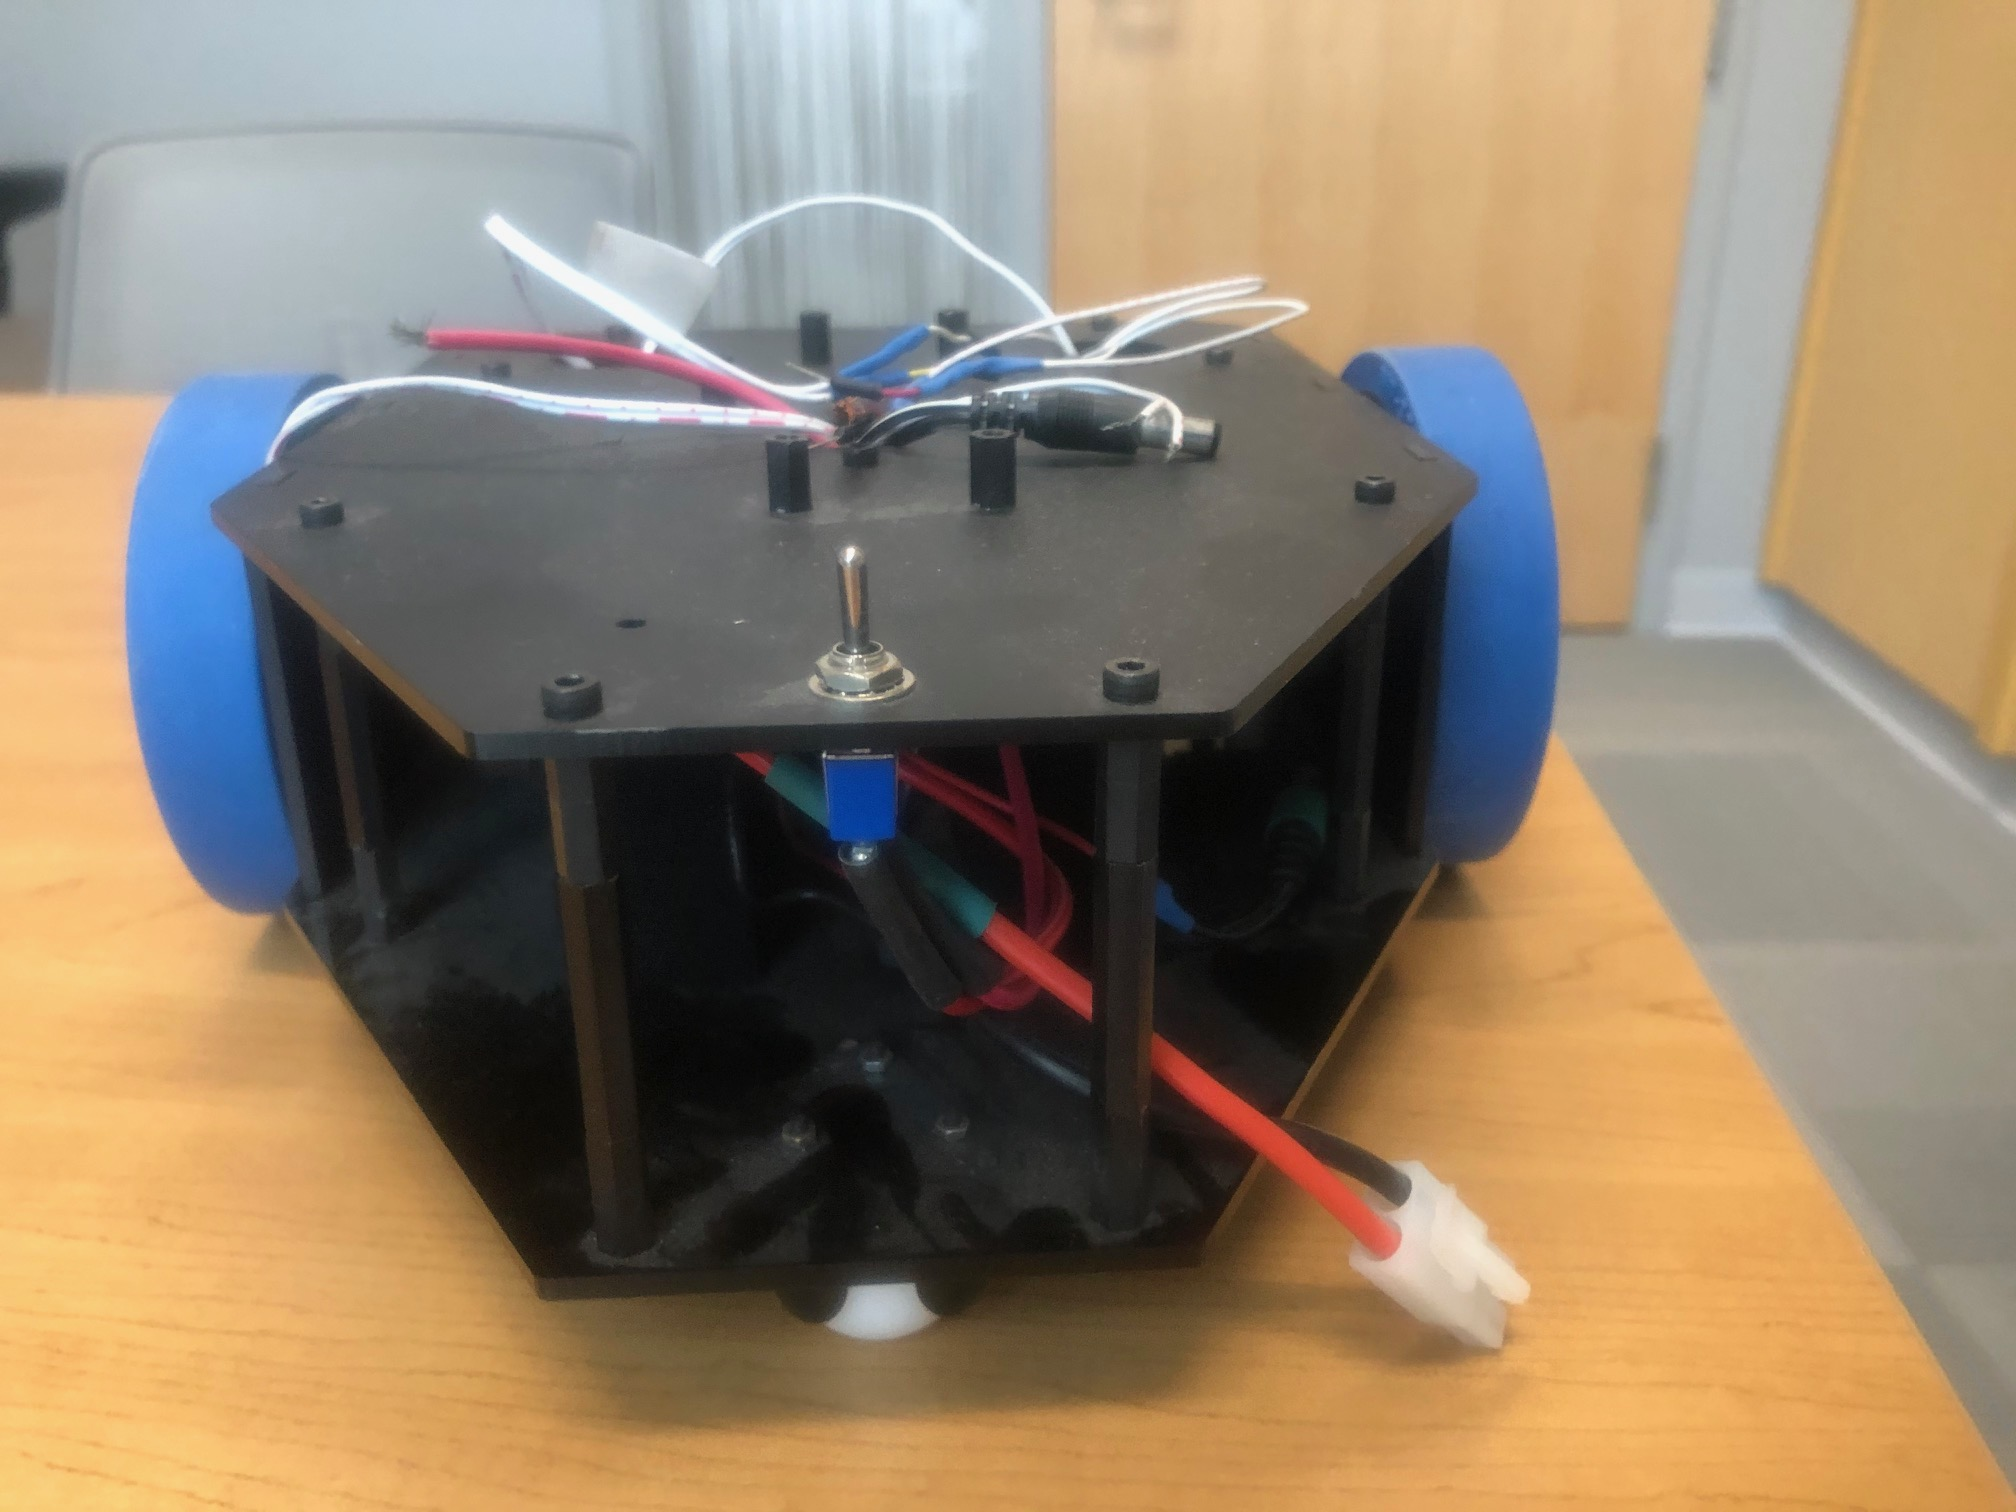
\includegraphics[width=4.5in]{figs/img/diffDriveChassis}
    \caption{Proposed Robot Chassis}
    \label{fig:diffDriveChassis}
\end{figure}

Finally, we discussed the parabolic reflector to directionalize the XBee sensor that will be mounted on the robot. Dr. Miah gave us the link to a previous senior project (\href{http://ee.bradley.edu/projects/proj2017/ekf_slam/Downloads/downloads.html}{found here}) that used such a parabolic reflector and directed us to the lab notebook for more information. We plan to look at the information there and decide whether to use the same design or to modify it.

%-------------------------------------------

\labday{Thursday, October 29, 2020}
\experiment{Budget Bot Evaluation}

JB\\
Today, we researched the Budget Bot chassis to see if it would be a better option than the Runt Rover. The motors included in the Budget Bot have a no-load speed of 212 RPM, and a rated load speed of 163 RPM. Since the wheels have a diameter of 3.875 inches (0.098425 m), the linear speed that can be achieved at 163 RPM is
$$v = r\omega = \left(\frac{0.098425}{2} [m]\right)\left(163 [RPM]\right)\left(\frac{1 [min]}{60 [s]}\right)\left(\frac{2\pi [rad]}{1 [rev]}\right) = 0.840 [m/s]$$
We would like to be able to reach a speed of at least 1 m/s, if possible. Then the loaded speed of the motor must be
$$\Omega_L = \left(\frac{1 [m/s]}{2\pi\frac{0.098425}{2} [m]}\right)\left(\frac{60 [s]}{1 [min]}\right) = 194 [RPM]$$
We found the Pololu 4751 motor on Digikey (\href{https://www.digikey.com/en/products/detail/pololu-corporation/4751/10450205}{here}) which has a no-load speed of 540 RPM at 12V. Since our batteries are only 7.4V, the no-load speed would be approximately $\frac{7.4}{12}(540 [RPM]) = 333 [RPM]$. This gives us a good tolerance for the effects of loading. However, these motors are somewhat expensive at \$39.95 each. We decided to ask Dr. Miah for his opinion on this.

\vspace*{12pt}
KA\\
In today's lab we researched a new robot chassis since we decided that the Junior Runt Rover robot model would not meet our requirements for this project. We continued to look at parts for the Budget Bot chassis and decided on better motors than what is already on the robot currently. After our initial update to the parts list we then delegated the project proposal content for the deadline on Tuesday, November 3. I decided to take the Title, Project Team, and Advisors, the Abstract, the Introduction, the Literature review, and the Bibliography/references.


\experiment{Project Proposal Planning}

JB\\
Today we divided out the tasks for the project proposal since the draft is due Tuesday, November 3. According to the information from Dr. Shastry, the proposal should have the following content:
\begin{enumerate}
    \item Title, Project Team, Advisors
    \item Abstract
    \item Introduction
    \item Literature review
    \item Expanded project statement
    \item Specifications of the system and the subsystems
    \item List of parts and complete specs of the parts needed
    \item List of tasks and task-sharing by the team members
    \item Timeline for accomplishing the tasks
    \item Include the following tasks:
    \begin{enumerate}
        \item Presentation to IAB members
        \item Final presentation
        \item Project demo
        \item Project report
    \end{enumerate}
    \item Bibliography and references
\end{enumerate}

Kalli will work on items 1 - 4 and 11. Darrah will work on items 5 - 7, and Jason will work on items 8 - 10.

%-------------------------------------------

\labday{Tuesday, November 3, 2020}
\experiment{Lab Time}

JB\\
Today we mostly worked on finalizing the parts list since it is due to Mr. Mattus. We also discussed the the usage of multiple XBees on the cart to reduce the time required to get signal strength readings from the remote. We decided to use four XBee modules mounted inside parabolic reflectors at 90 degree increments. We also decided to use a fifth XBee on top of the reflectors to broadcast the signal strength query to the remote.

\vspace*{12pt}
KA\\
In today's lab we reviewed the project proposal for the senior project meeting today. After we went over the paper we researched the best design which is to have four parabolic reflectors which would make it easier to pick up the stronger signal from the remote device and increase the XBee's resolution. We also finalized the parts list for our project and sent it to Mr. Mattus so that the parts could be ordered. I left the lab a few minutes early in order to pick up the Budget bot chassis from Dr. Miah and start working with the new model.

\experiment{Meeting Minutes}
Agenda: 
\begin{itemize}
    \item Parts
    \begin{itemize}
        \item Quantities - Should we just build 1 cart next semester to cut back on costs?
        \item Reflector - Parabolic or Paraboloidal
        \item Guidelines on using personal parts
    \end{itemize}
    \item Revised Specifications
    \begin{itemize}
        \item Make obstacle avoidance a stretch goal
        \item Make status LEDs and buttons a stretch goal
    \end{itemize}
    \item Go over proposal draft
\end{itemize}

JB\\
In today's meeting, we decided that we will only build two robots in order to limit the cost of the project. We also decided to use parabolic reflectors similar to the one shown in \autoref{fig:reflectorExample}. We discussed the construction of such a reflector, and decided to design a parabolic frame about 15cm across. We will print this frame on a 3d printer, and line the inside with aluminum foil tape to make it reflective.

\begin{figure}[h!]
    \centering
    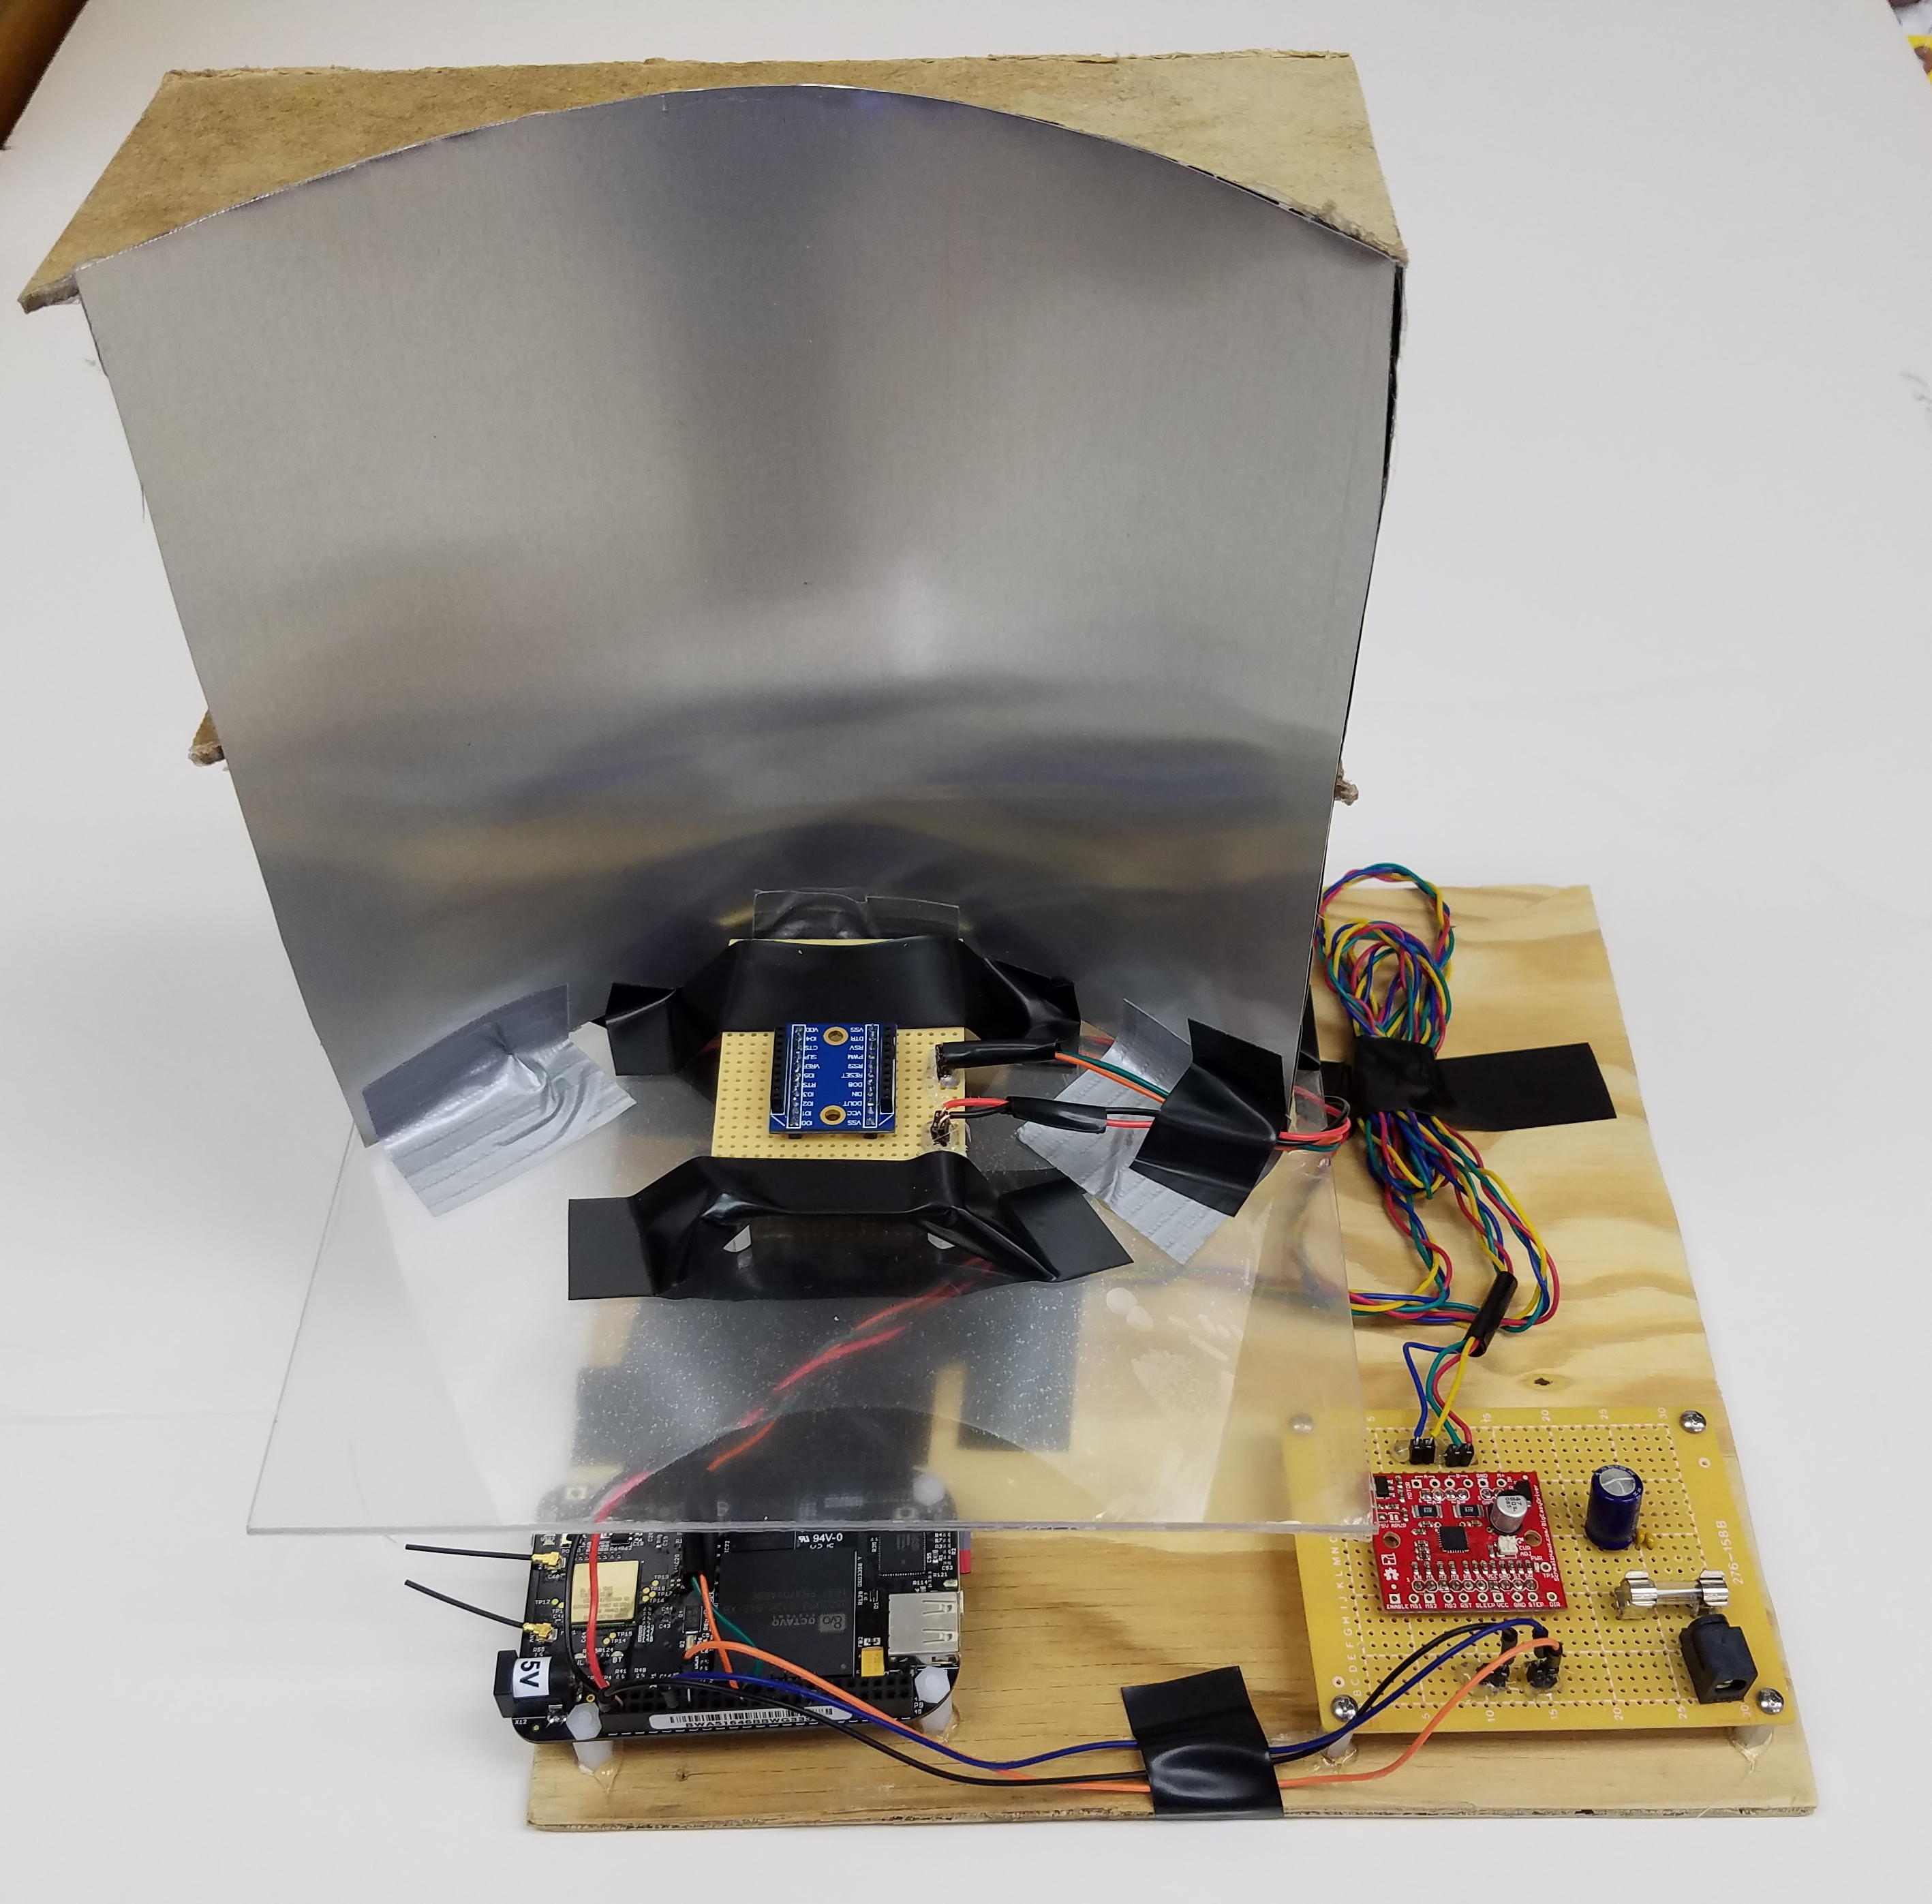
\includegraphics[width=4.5in]{figs/img/customizedRadioTransceiver}
    \caption{Parabolic Reflector Example}
    \label{fig:reflectorExample}
\end{figure}

%-------------------------------------------

\labday{Thursday, November 5, 2020}
\experiment{Lab Time}

JB\\
Today I worked on creating a CoppeliaSim model of the Budget Bot robot. I got the model created, and I am able to send commands from Matlab. However, at this point, commanding 0.25 m/s for 4 seconds results in the robot traveling about 1.25 m instead of just 1 m. I am not sure why it is doing this.

\vspace*{12pt}
KA\\
Today I worked on putting together the project proposal presentation slides that are due on Tuesday, November 10. I got through the system requirements and then looked for images to put in this part. I will need input from Jason once his CoppeliaSim model is done so that I can add the model to the slides. I will continue to work on the slides and have them ready for review in the lab day on Tuesday, November 10. 

%-------------------------------------------

\labday{Tuesday, November 10, 2020}
\experiment{Lab Time}

JB\\
Today I worked on the CoppeliaSim model of the Budget Bot robot. I was able to get the model to successfully complete the point navigation task for a static point. Then I worked on updating the simulation to have the model follow a moving target. I used \autoref{alg:navAlgo} to accomplish this.

\begin{algorithm}[h!]
    \SetAlgoLined
    \KwIn{Signal Strengths from Remote}
    \KwOut{Mobile Robot Trajectory}
    \Begin
    {
        Initialize robot pose $q_0 = [x_0, y_0, \theta_0]^T$\\
        Initialize parameters, sampling time $T > 0$, following distance $d_f$, $K_p$, $K_\omega$\\
        \While{true}{
          Estimate distance $d_{Ref}$ to remote using signal strength\\
          Estimate angle $\theta_{Ref}$ to remote using signal strengths\\
          Compute coordinates of target point with respect to robot's local frame as $x_{Ref} = (d_{Ref} - d_f)\cos \theta_{Ref}$, $y_{Ref} = (d_{Ref} - d_f)\sin \theta_{Ref}$\\
          Compute linear speed $v(t) = sign(x_{Ref})K_p\sqrt{x_{Ref}^2 + y_{Ref}^2}$\\
          Compute $\omega(t) = K_\omega \theta_{Ref}$\\
          Compute left and right wheel speeds for robot\\
          Apply wheel speeds to robot\\
        }
    }
    \caption{Remote Following Algorithm}
    \label{alg:navAlgo}
  \end{algorithm}

\vspace*{12pt}
\vspace*{12pt}
KA\\
In today's lab I worked on touching up the project proposal slides with the revisions from Jason and Darrah. I needed to fix a few figures and had Jason help me with resizing the gantt chart for the project timeline. In the remaining lab time I helped Jason with some minor issues he had in his CoppeliaSim model and worked on implementing the model and code he created on my own computer.

\experiment{Meeting Minutes}
Agenda: 
\begin{itemize}
    \item Go over proposal
    \item Discuss simulation
\end{itemize}

JB\\
In today's meeting, we discussed the current status of the simulation. The robot was not following the remote correctly, but it was following somewhat. We determined that we should get the simulation to work in the ideal, noise-free scenario first. After that is working we will add noise. Dr. Miah also told us to create a video to show at the beginning of the presentation.

%-------------------------------------------

\labday{Thursday, November 12, 2020}
\experiment{Lab Time}

JB\\
Today I worked on coming up with a way to simulate the angle estimation that we plan to use. We discussed methods of determining what the signal strength should be for the receivers in the reflectors based on the angle to the remote. We determined that we should use some form of the cosine of the angle between the receiver and the remote to determine what the signal strength should be. We also discussed the shape of the reflectors. Since the remote is likely to be higher than the receivers under normal usage, a strictly paraboloidal shape (see \autoref{fig:paraboloidalReflectors}) may not work correctly. We thought that a paraboloidal shape below the antenna and a parabolic shape above the antenna (see \autoref{fig:paraboloidalParabolicReflectors}) might work better. I worked on creating a 3d model of the reflectors to use in CoppeliaSim so we can see the rotation of the reflectors on the top of the robot.

\begin{figure}[h!]
    \centering
    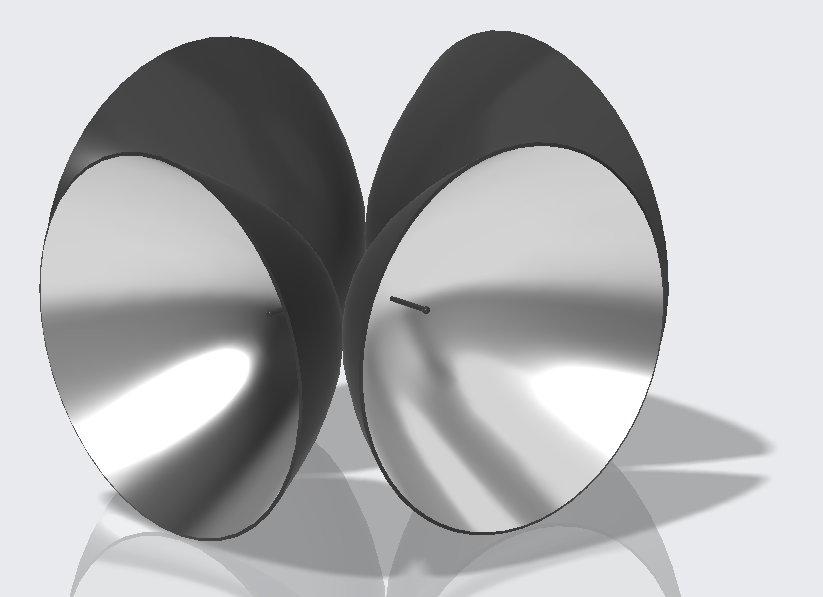
\includegraphics[width=4.5in]{figs/img/paraboloidalReflector.png}
    \caption{Paraboloidal Reflectors}
    \label{fig:paraboloidalReflectors}
\end{figure}

\begin{figure}[h!]
    \centering
    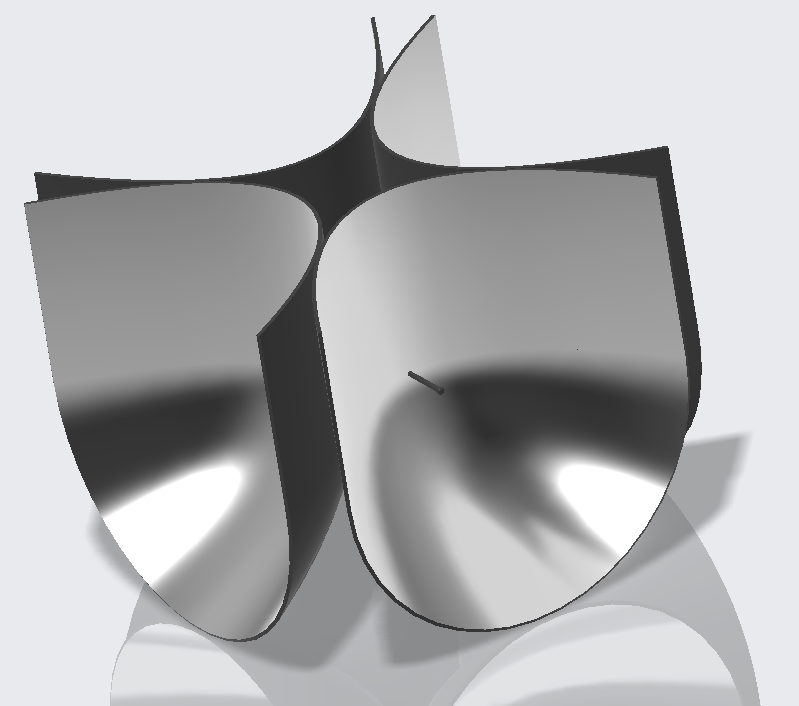
\includegraphics[width=4.5in]{figs/img/parabolicReflector.png}
    \caption{Paraboloidal/Parabolic Reflectors}
    \label{fig:paraboloidalParabolicReflectors}
\end{figure}

\vspace*{12pt}
\vspace*{12pt}
KA\\
Today in the lab time Jason demonstrated his CoppeliaSim model and we were able to see that the robot tracks to the point while following the remote in a circular path with some added noise. After the demo of the CoppeliaSim model I decided to research some ways of modeling the parabolic reflector in Matlab and found this website as a reference: \href{https://www.mathworks.com/help/antenna/ug/pattern-analysis-of-the-symmetric-parabolic-reflector.html}{https://www.mathworks.com/help/antenna/ug/pattern-analysis-of-the-symmetric-parabolic-reflector.html}. After we discussed this code as a group we decided to try a different method of modeling the parabolic reflector since the code did not allow for us to change the parameters to what we needed for our project.

%-------------------------------------------

\labday{Tuesday, November 17, 2020}
\experiment{Lab Time}

JB\\
In today's lab time, we worked on the proposal document and presentation. I worked on creating an introductory video for the start of the presentation.

\vspace*{12pt}
KA\\
In the lab today we worked on the project proposal presentation slides to finalize it for the presentation and did a practice run of the presentation.

\experiment{Meeting Minutes}
Agenda: Go over proposal

JB\\
In today's meeting, we discussed the proposal and proposal presentation. We found that there were two bibtex warnings when the proposal was compiled. Dr. Miah gave us the following recommendations for the document:
\begin{itemize}
    \item Add a few sentences before the first subsection in the Functional Requirements section
    \item Include the list of parts
    \item Add color to the block diagrams
    \item Include a flowchart and pseudo-code of the algorithm
    \item Include the images of the reflector models
\end{itemize}

In addition, Dr. Miah gave us the following recommendations for the presentation:
\begin{itemize}
    \item Use figures in most of the slides
    \item Use less text, rather than more
\end{itemize}

%-------------------------------------------

\labday{Thursday, November 19, 2020}
\experiment{Lab Time}

JB\\
In today's lab time, we worked on the proposal document and presentation.

\vspace*{12pt}
KA\\
In the lab today I worked on putting more pictures into the slides and worked on the corrections Dr. Miah suggested on Tuesday. I fixed the bibliography file with the updated sources for the pictures. I also changed the references in the paper.

%-------------------------------------------

\labday{Tuesday, December 1, 2020}
\experiment{Lab Time}

JB\\
In today's lab time, we worked on the proposal document and presentation.

\vspace*{12pt}
KA\\
We went over the presentation slides in the lab time today to fix any last minute mistakes or issues. I went through the three references used in the references to add more to my part of the presentation and created an outline for my speaking parts to better perfect my speech.

\experiment{Meeting Minutes}
Agenda: Go over proposal

%-------------------------------------------

\labday{Tuesday, December 1, 2020}
\experiment{Meeting Minutes}

JB\\
Today was the last day of classes for the semester. We just briefly met to
discuss the results of the proposal presentation and our plans for Christmas
break.

\labday{Thursday, January 28, 2021}
\experiment{Meeting Agenda}

SM\\
\begin{itemize}
  \item Weekly meeting schedule

  \item Plan including timeline and milestones  on implementing the theoretical work developed for ECE 498

  \item Plan for Student expo posters/IAB posters     

\end{itemize}

\experiment{Meeting Minutes}

JB\\
Today we met to kick off the spring semester of senior project. We decided to have our weekly meetings with Dr. Miah and Dr. Shastry on Thursdays from 2 to 3 pm. We were instructed to find some scheduled time to work together in the laboratory. We also discussed the poster for the IAB and the Student Expo. We will be making a poster presentation for the IAB, and it is strongly recommended to present at the Student Expo. Dr. Miah reminded us that we should be working on the implementation during this lab time. He also told us to focus on getting the robot to move toward the remote with a minimum number of features (no LEDs, buttons, etc). Once the main goal of the project is completed, we can add more features if we have time.

\labday{Monday, February 1, 2021}
\experiment{Meeting Time Update}

JB\\
We are supposed to spend at least 6 hours per week working in the lab. We have decided to meet from 12 - 2 pm on Tuesdays and Thursdays. This gives us 4 hours of lab time together. We will individually go to the lab for the remaining 2 hours per week.

\labday{Tuesday, February 2, 2021}

\experiment{XBee Configuration}

JB\\
Today we worked on connecting the XBees with XCTU and setting them up for our purposes. We did not get it completely figured out yet. We are thinking that we will need to run all of the XBees on the robot as coordinators, and the remote as an endpoint.

Today we also got the rest of our parts from Mr. Mattus and tried out the Budget Bots he set up for us. As of now, we are not able to run the motors by plugging the DC jack from the battery into the BeagleBone. The suspicion is that it does not work since the battery is only 7.2 V, while the DC input port expects 12 V.

\vspace*{12pt}
KA\\
During the lab time I downloaded XCTU in order to learn how to run the program and communicate with the XBees. Darrah helped Jason and I understand some of the setup of XCTU and how to connect the XBee and write commands to it. For the one hour independent lab time I worked on trying to run XCTU with my own XBee and was able to follow the steps Darrah went through in the lab. I only had one issue with the initial connection to the XBee but was able to get past it. 

\labday{Thursday, February 4, 2021}
\experiment{XBee Configuration}
JB\\
Today I worked on configuring the XBees again. Kalli found a link that helped get two XBees communicating with each other (\href{https://www.digi.com/resources/documentation/Digidocs/90002126/tasks/t_configure_remote_devices.htm}{link}). I got two XBees configured in a way that I was able to request signal strength readings from the remote XBee. I tested this with the remote in various parts of the room and verified that the signal strength changed with distance.

\vspace*{12pt}
KA\\
In today's lab Jason and I worked on putting together the remote XBee circuit and added an LED indicator to test if power was going to the XBee. Once we connected the remote XBee to XCTU Jason then was able to test signals back and forth using another XBee. While Jason tested the XBees I made a second XBee remote for back-up. During the independent hour of lab time I reconfigured one of the budget bots to see where we could move the breadboard in order to make room for the stepper motor. 

\experiment{Meeting Agenda}
JB\\
\begin{itemize}
    \item Project status update
    \item Code location
    \item Multiplexer for connecting with receiving XBees
\end{itemize}

\experiment{Meeting Minutes}
JB\\
Today we met with Dr. Miah in the lab. We discussed the status of the project so far. The battery packs with the Budget Bots connect to the BeagleBone Blue through the 12V jack. This does power the BBBlue, but it does not power the motor drivers. Rather than using external circuitry to control the motors, we decided to use LiPo batteries instead, and connect them to the built-in battery port on the BBBlue. I had a LiPo battery available from a previous class, so we tested this and verified that we can run the motors from this battery. We decided to remove the existing batteries from the Budget Bot and use LiPo batteries instead.\vspace{12pt}

Another issue we discussed was how to mount the stepper motor. The bracket that I had 3d printed for this purpose used the four screws at the back of the Budget Bot for mounting. However, Mr. Mattus mounted a breadboard in that space since he did not know we needed to put the stepper motor there. We came up with two options:
\begin{itemize}
    \item Make a raised bracket to allow the stepper motor to be mounted above the breadboard
    \item Move the breadboard to the front panel of the Budget Bot Chassis
\end{itemize}
We will discuss these options with Mr. Mattus to determine how to proceed.\vspace{12pt}

We have also discovered that we really only have access to 3 UART ports and one USB port on the BBBlue. However, we need to connect 5 XBee modules. We decided the best option would be to use a multiplexer to be able to switch between the 4 XBees in the reflectors. That way we could use one UART port for those 4 XBees and another UART port for the transmitter XBee. We will ask Mr. Mattus for such a multiplexer.\vspace{12pt}

Finally, we decided to create a Code folder in the Git repository to contain and track all of our code files.

\labday{Tuesday, February 9, 2021}
\experiment{Lab Time}
KA\\
In today's lab time we worked on configuring multiple XBees to send and receive signals. We split up the work and I looked up the current output for the motor drivers and the current output for the GPIO ports on the BeagleBone Blue. I found three datasheets that I uploaded to the project google drive under the data sheets folder for future reference.

\begin{itemize}
    \item 4 motor ports - 1.2A average output with a 3.2A possible peak
    \item GPIO ports - a source of 6mA, a sink of 8mA, and some pins are limited to 4mA
    \item XBee modules (TH) - transmit current of 45mA and an idle/recieve current of 31mA
\end{itemize}

I also found a helpful resource from Matlab, (\href{https://www.mathworks.com/help/supportpkg/beagleboneio/examples/working-with-beaglebone-black-hardware.html}{link}), about the hardware of the BeagleBone Black which is similar to the BeagleBone Blue and listed the maximum permitted current draw from the 3.3V power source which is 50mA.\vspace{12pt}

JB\\
Today I first crimped some pins to the ends of one 6-pin and two 4-pin JST connectors to make it easier to hook up the XBees to the BBBlue. Then I worked on redesigning the reflectors to orient the XBee antennae vertically, as well as to make the reflector array modular (allow removal of a single reflector dish). Today I also talked to Mr. Mattus about the extra XBee adapters, the multiplexers, and the stepper motor mounting. He gave me two more XBee adapters, but they do not have mounting holes. I can make a mounting mechanism where the adapter is held down by a bar that is screwed onto the frame, but this will not give connection to GND for making a ground plane beneath the transmitter XBee. Mr. Mattus informed me that he does not have any multiplexers like we need, so he will order some DG409DJ+ multiplexers. Regarding the stepper motor mounting, we decided that the best option for now is to move the BBBlue to one side of the Budget Bot and move the breadboard adjacent to it. This frees up the space at the back of the Budget Bot for mounting the stepper motor with a bracket like the one I already made.


\labday{Wednesday, February 10, 2021}
\experiment{Stepper Motor Control}

JB\\
Today I wrote a piece of test code for the stepper motor to rotate back and forth 90\textdegree. This worked successfully. I created a code folder in the repository and placed stepTest.c inside.

\labday{Thursday, February 11, 2021}
\experiment{Lab Time}
JB\\
Today Kalli and I lined the inside of two of the new reflectors with foil tape. Then we connected wires to two XBee adapter boards for power and serial communcation. Then we mounted these adapter boards inside the reflectors and put XBees in them. After that I worked on writing a library for the stepper motor control.

\vspace*{12pt}
KA\\
In the lab I helped Jason with applying the foil tape to the parabolic reflectors and assembled the XBees into the reflectors. After helping Jason I worked with Darrah on assembling the multiplexer substitute with transistors in order to start testing multiple XBees.

\experiment{Meeting Agenda}
JB\\
\begin{itemize}
    \item New reflector dish design
    \item Transmitter XBee mounting
    \item Current limits
    \begin{itemize}
        \item XBee power
        \item Motor power
    \end{itemize}
\end{itemize}

\experiment{Meeting Minutes}
JB\\
In today's meeting, we discussed the new reflector design. Dr. Shastry pointed out that we are not actually designing a dish antenna. Rather, we are just designing a reflector to enhance the signal received. The paraboloidal shape is just used to focus the signal on one point. We also discussed a ground plane beneath the transmitter XBee on top of the reflector array. Since the new XBee adapters we got from Mr. Mattus do not have mounting holes on them, it will be more difficult to connect the ground plane to the ground of the XBee. Dr. Shastry told us not to worry about that. Next we discussed the power requirements of the XBees. We had found that the power from the UART ports can only supply 50 mA, while each XBee requires 31 mA while idling and 45 mA when transmitting. We decided to try making a separate power circuit for the XBees by connecting a 3.3V regulator to the battery, putting a $10\mu F$ capacitor across the output, and powering the XBees from that. Finally, we discussed the current requirements of the DC motors. The motors have a stall current of around 4A, but under normal operation, the current is much less. The motor drivers on the BBBlue are rated for 1.2A average, with a peack of 3.2A. We decided to investigate the possibility of using external H-bridges, but also to just keep using the BBBlue ports to see if anything burns out.

\labday{Thursday, February 18, 2021}
\experiment{Lab Time}
JB\\
In the lab today, we finished putting foil tape on the remaining reflectors and the top plate. Then I assembled the reflector array and mounted it on the robot.

\vspace*{12pt}
KA\\
Today I helped Jason put foil tape on the remaining two reflectors and add the XBees to them as well. I assisted Darrah with the multiplexer circuit since the last circuit needed to be redone. Darrah explained to me how the transistor circuit worked and when we got errors in the sent messages to the XBees we went through the circuit to find where the error was occurring. The image of this circuit can be seen in Figure \ref{fig:transistor_circuit}.

\begin{figure}
    \center
    \includegraphics[width=5in]{figs/multiplexer_draft_circuit.jpg}
    \caption{Working draft of the transistor circuit}
    \label{fig:transistor_circuit}
\end{figure}

\experiment{Meeting Agenda}
JB\\
\begin{itemize}
    \item Status update
    \item Clarify motor power
\end{itemize}

\experiment{Meeting Minutes}
JB\\
In today's meeting, we discussed the current status of the project. We have the reflector array completed. At this point, we are waiting on the multiplexer chip to be able to complete the robot. We discussed this and decided to check with Mr. Mattus whether it has been ordered yet. If not, we will just order it ourselves and pay from our own pocket. We also clarified that we are going to try controlling the motors directly from the BBBlue's built-in H-bridges as well as trying with external H-bridges.

\labday{Tuesday, February 23, 2021}
\experiment{Lab Time}
JB\\
Today I got the new batteries and multiplexers from Mr. Mattus. I created a new wiring harness with a Deans connector to allow us to supply power to the XBees external to the BBBlue. After completing that, we tested the multiplexers to make sure they functioned as desired. We were able to send UART messages through the multiplexer and switch between different channels. Some images of the robot in its current state are shown in Figures \ref{fig:robot1} - \ref{fig:robot3}.

\begin{figure}
    \center
    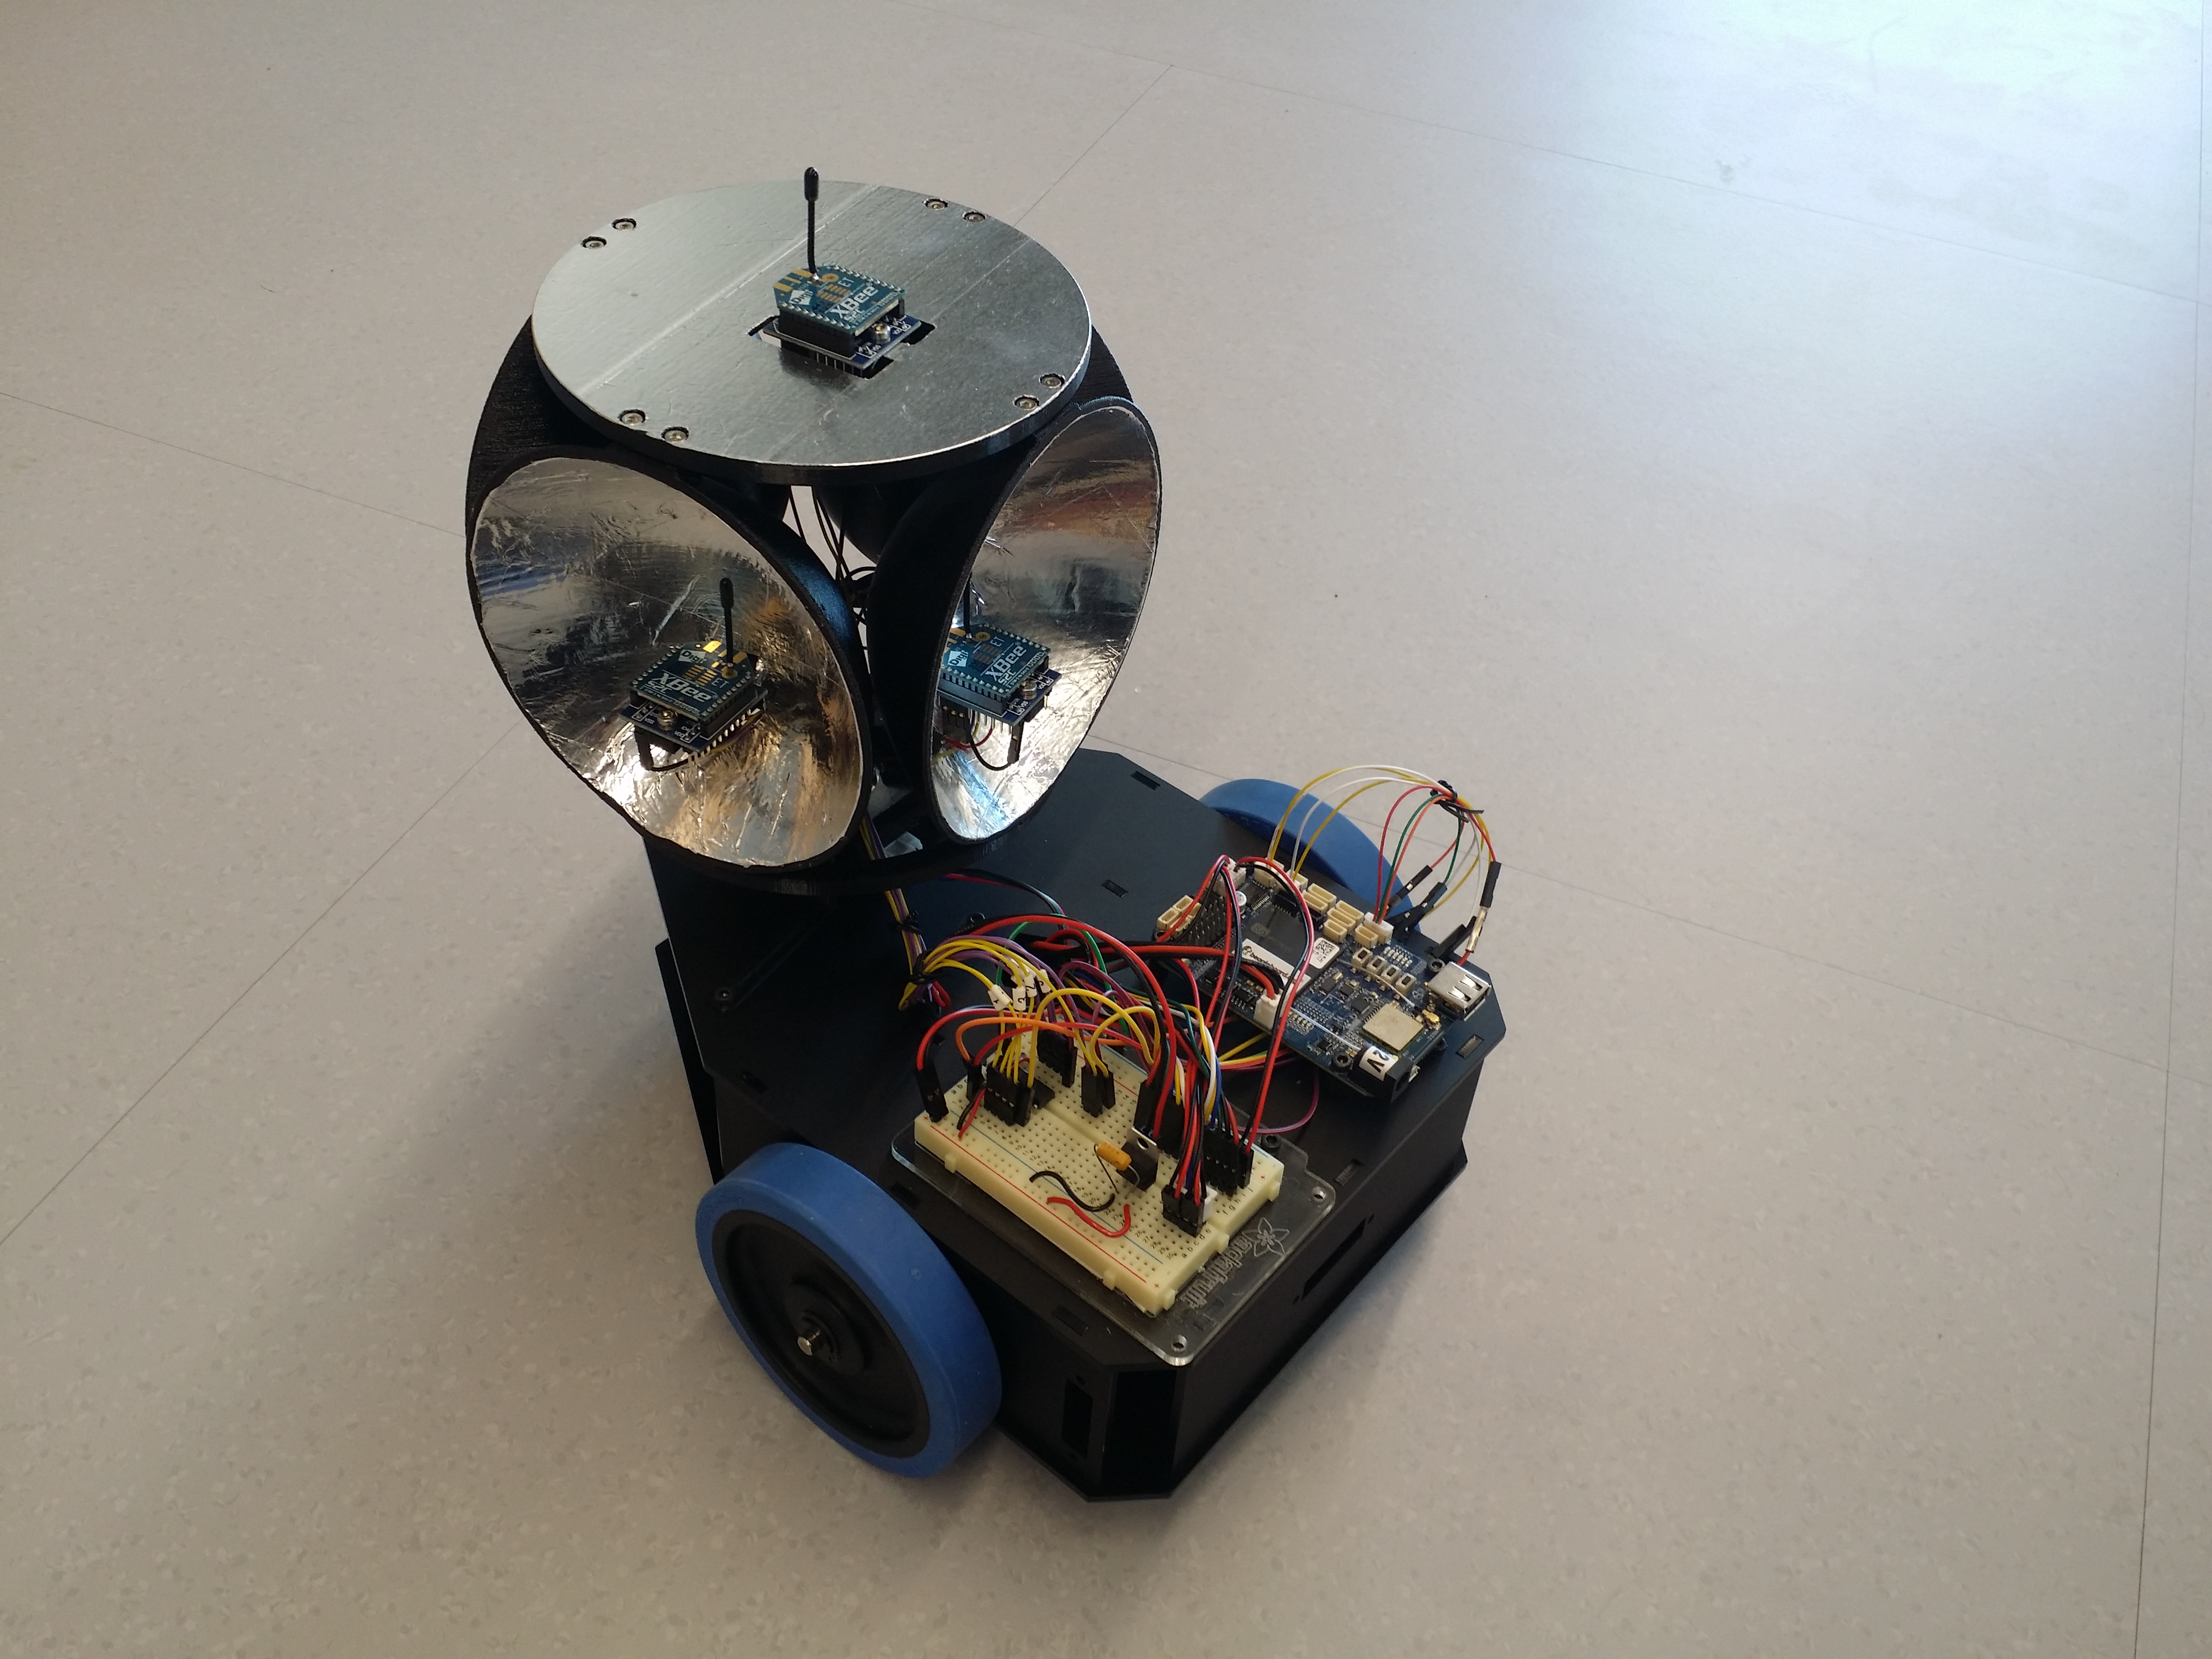
\includegraphics[width=4.5in]{figs/img/robot1.jpg}
    \caption{Current State of Robot}
    \label{fig:robot1}
\end{figure}

\begin{figure}
    \center
    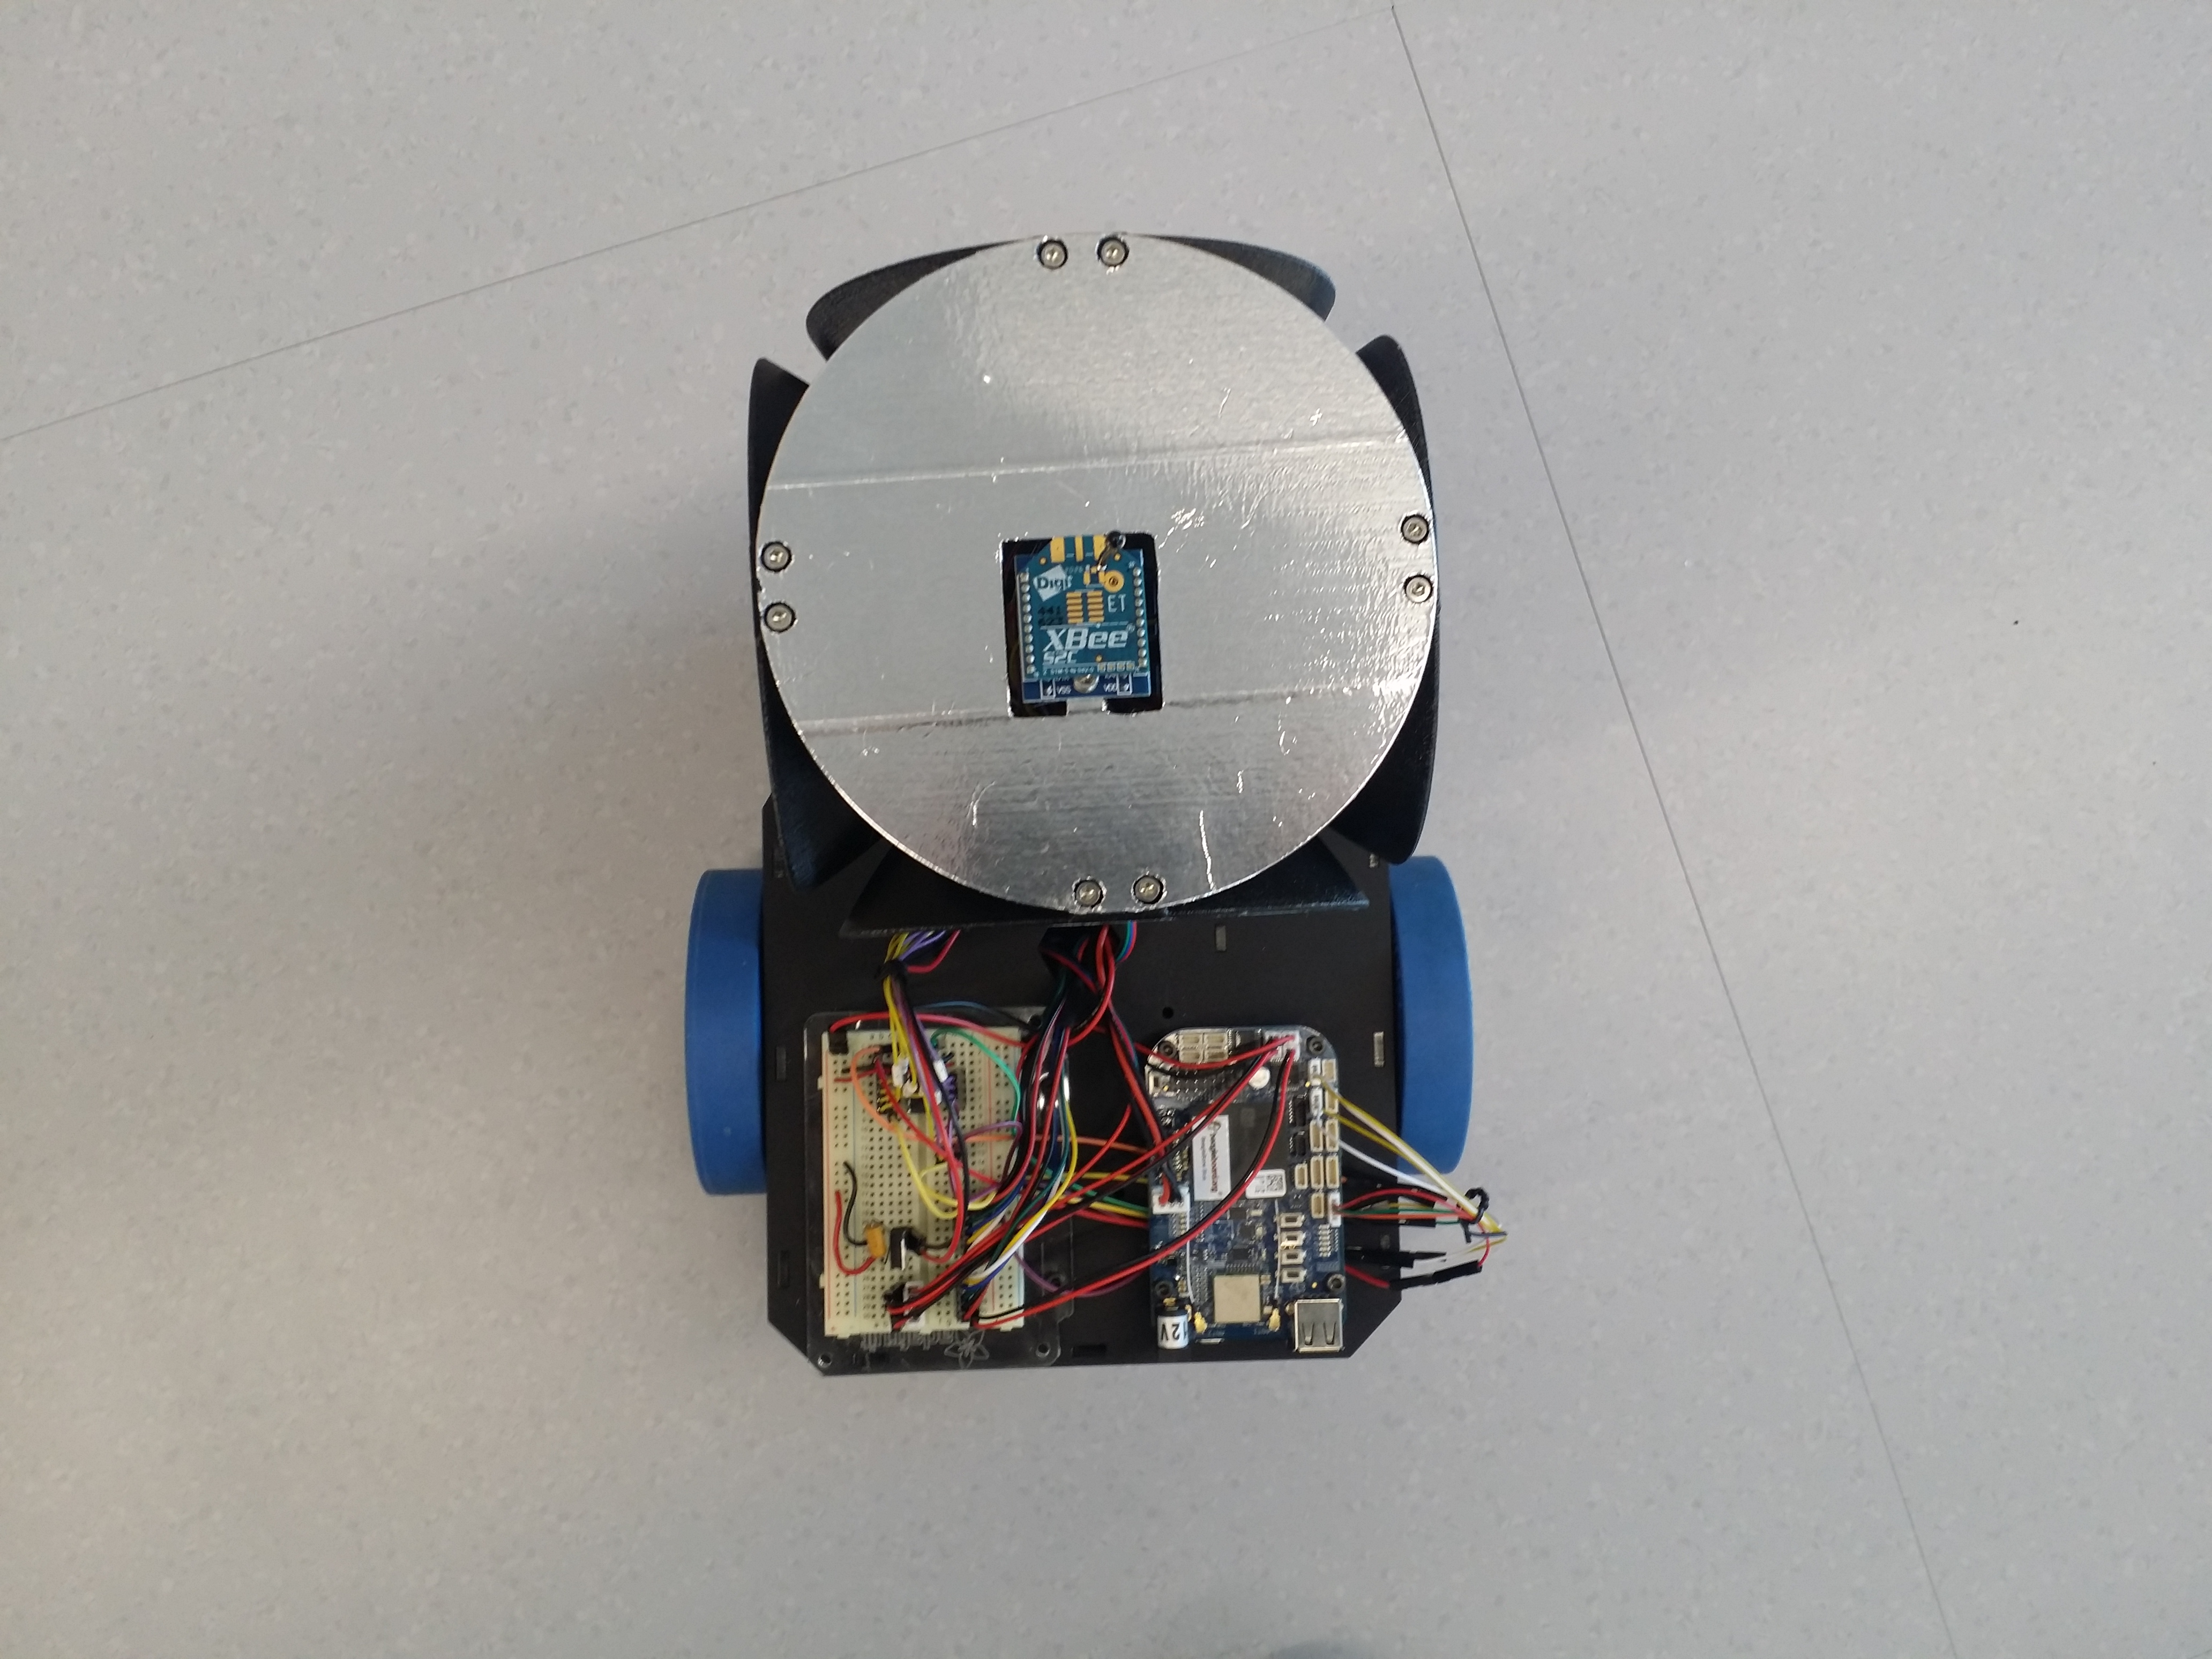
\includegraphics[width=4.5in]{figs/img/robot2.jpg}
    \caption{Current State of Robot}
    \label{fig:robot2}
\end{figure}

\begin{figure}
    \center
    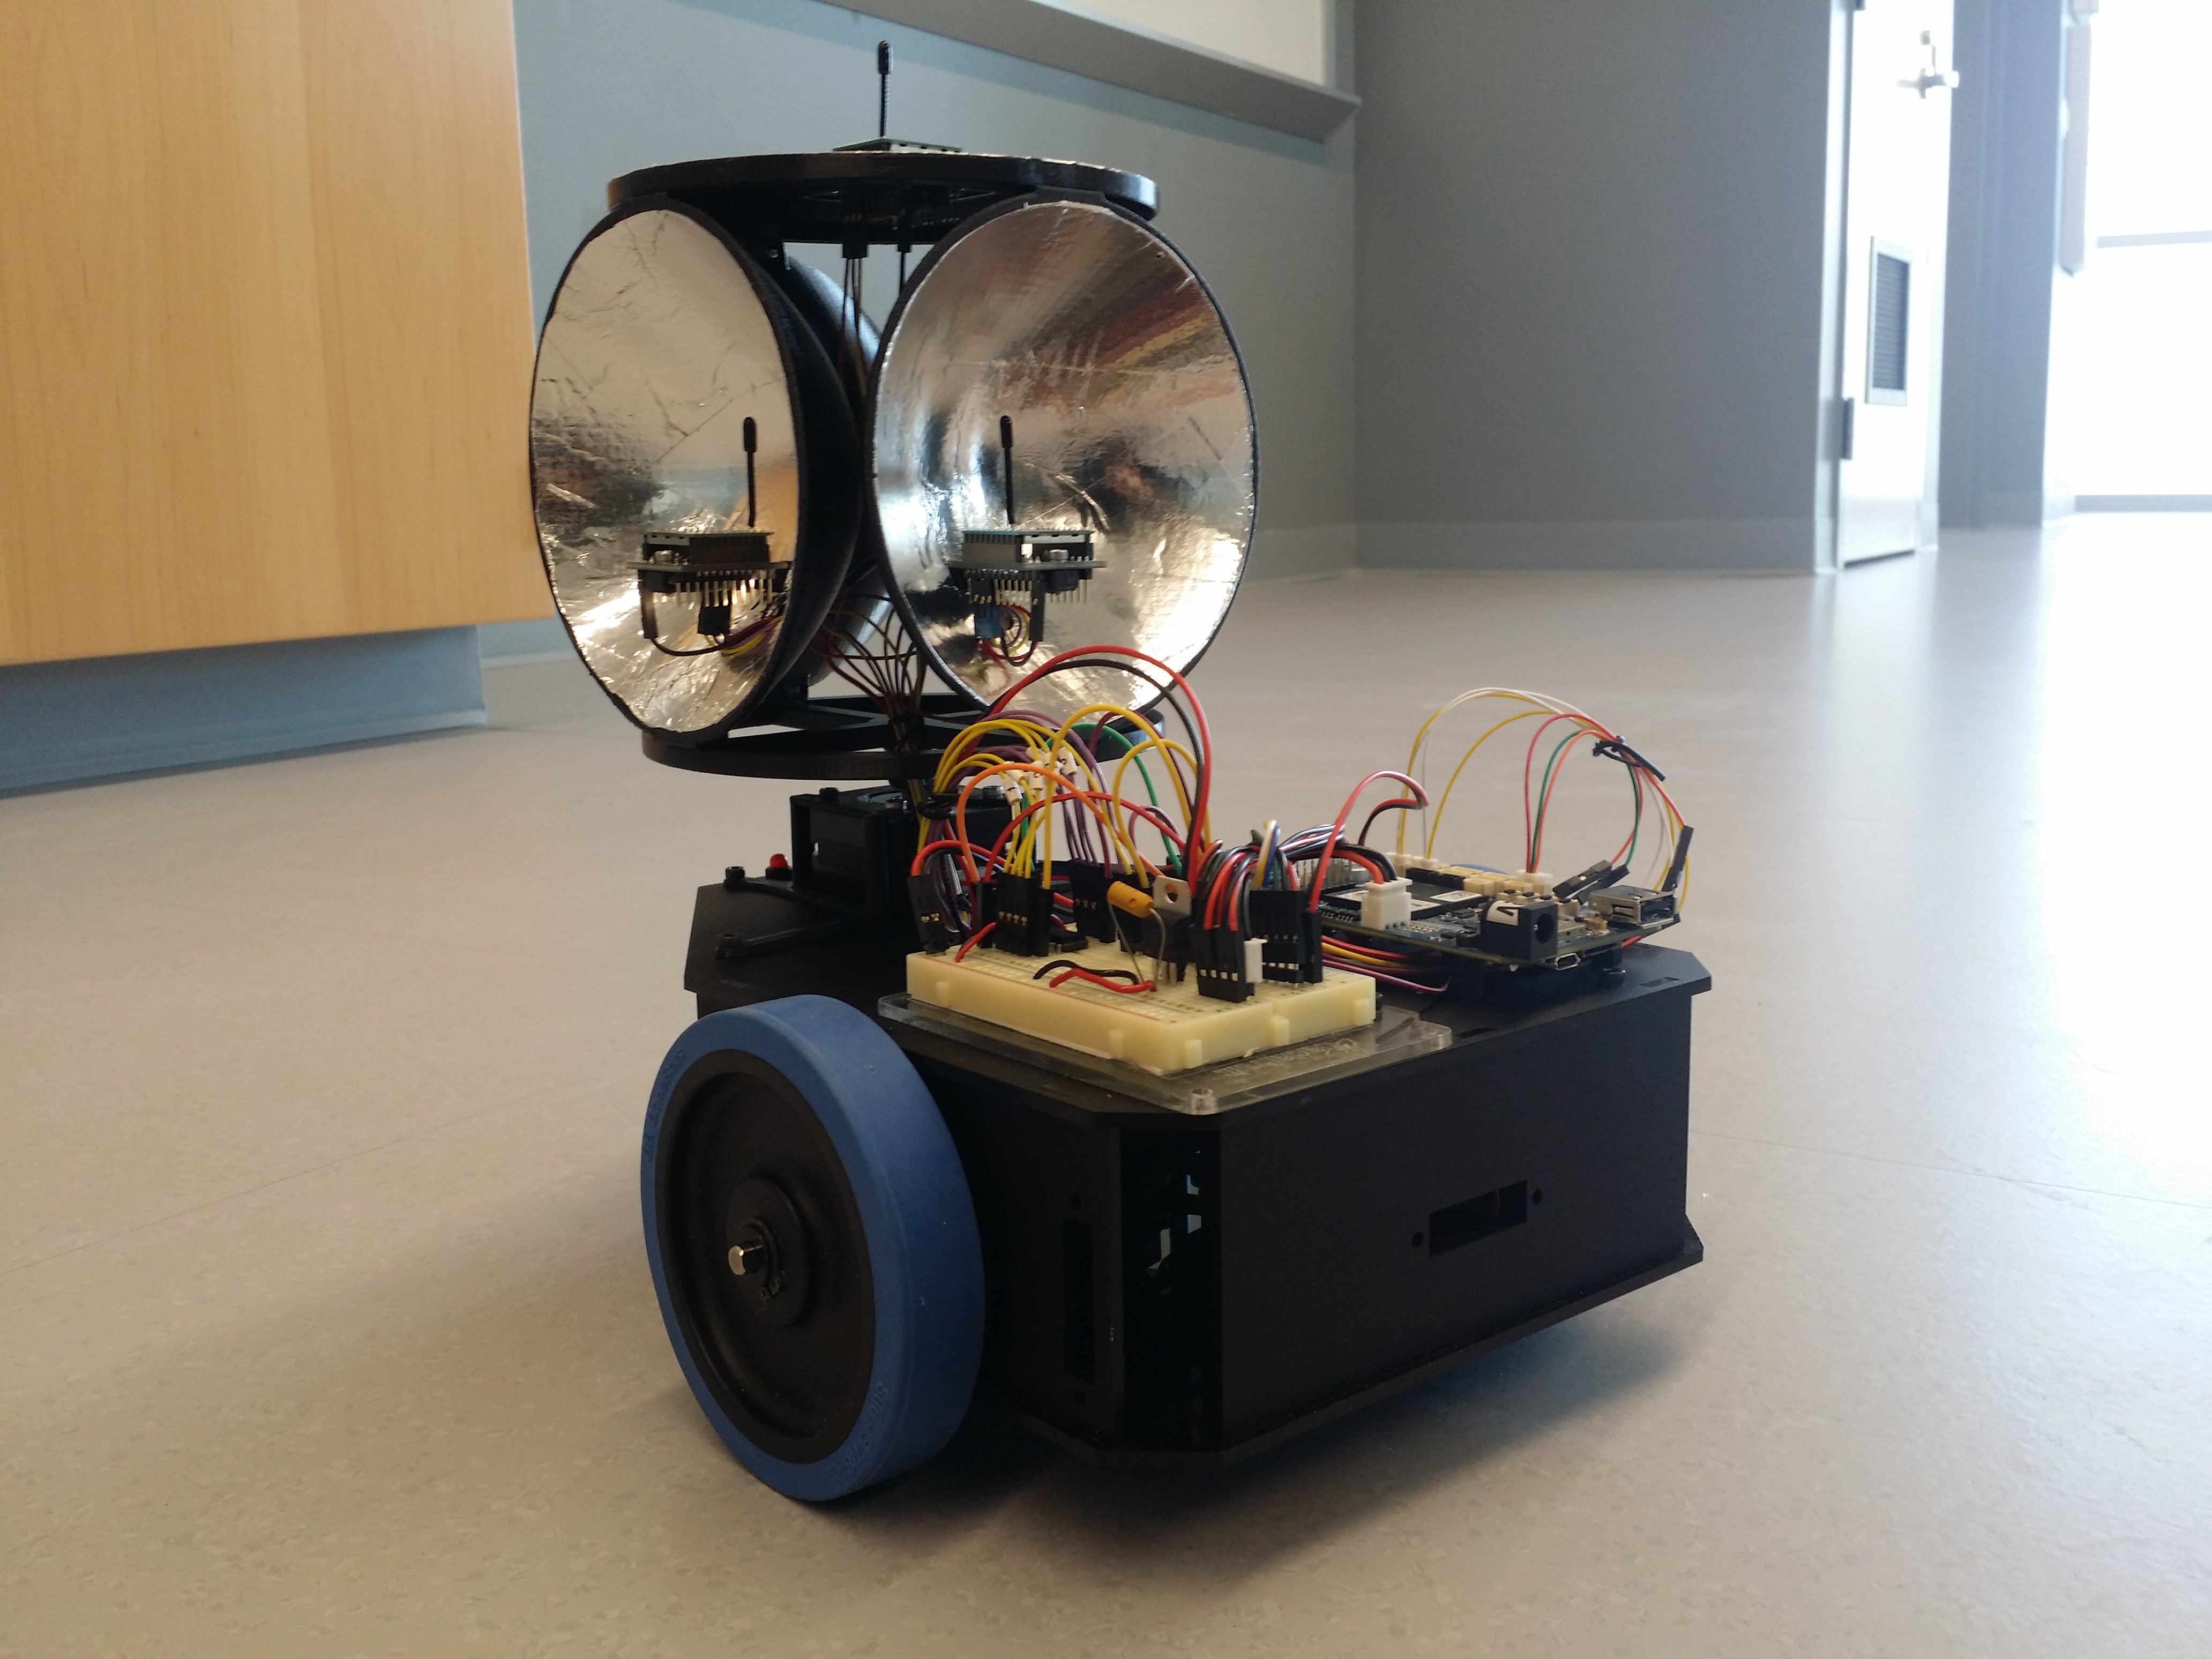
\includegraphics[width=4.5in]{figs/img/robot3.jpg}
    \caption{Current State of Robot}
    \label{fig:robot3}
\end{figure}

\labday{Thursday, February 25, 2021}
\experiment{Lab Time}
JB\\
Today in the lab we tested the multiplexer with the XBees. We were able to successfully send a request to the remote and read the strength from all of the XBees using the multiplexer to switch between them. I also updated the stepper library some.

\vspace*{12pt}
KA\\
In today's lab we worked on getting the multiplexer working on the robot so that we could run the test code Darrah developed for multiple XBee communication. We had a few minor issues with the code but we were able to solve them and made good progress on speeding up the response time for communication between the XBees.

\experiment{Meeting Minutes}
JB\\
We did not have a formal meeting today. We just met in the lab and discussed the status of the project briefly, then used the rest of the time to actually work on the project.

\labday{Tuesday, March 2, 2021}
\experiment{Lab Time}
JB\\
In today's lab we wrote code to find the distance and angle of the remote. We are taking signal strength measurements every 9 degrees. Therefore, we are taking 10 measurements for each full 90\textdegree~sweep of the reflector array. The average of the strengths received by the top XBee is used to calculate the distance. To calculate the angle, we are computing a value by adding the strength at each index of the strengths array and 0.5 times the strength on either side. Then the index where we got the maximum value is assumed to be the direction of the remote. We tested this code, and the distance measurement is somewhat reasonable. However, the angle measurement is not correct.

\vspace*{12pt}
KA\\
In today's lab we worked on collecting signal strength data from the XBee's when rotating the reflector array. We ran the code to test this function and changed a few variables to see what worked best in received signal strength.

\labday{Thursday, March 4, 2021}
\experiment{Angle Estimation}
JB\\
In today's lab, we worked on tuning the angle estimation. We sampled a bunch of signal strength data points to see how consistent our results were. They were not very consistent. However, we realized that in our previous code, we were finding the maximum of the values received. Since these values are actually path loss, we need to instead find the minimum. We updated the code to do that, and the angle estimation is giving somewhat ok results.

\vspace*{12pt}
KA\\
In today's lab we worked on angle estimation and taking samples of signal strength data in order to get a rough estimate of the angle the remote was at. This was a work in progress but towards the end of the lab session we were able to get some promising results from the code. After the lab session Jason and I stayed behind to work on putting together the second robot in order to use it for multiple code fixes rather than all three of us trying to work on code on a single BeagleBone Blue.

\experiment{Meeting Agenda}
KA\\
\begin{itemize}
    \item Status update
    \item Student Scholarship Expo
\end{itemize}

\experiment{Meeting Minutes}
JB\\
In today's meeting, we discussed the current status of the project. We are able to get a somewhat ok estimate of the angle of the remote. However, the distance estimate spikes drastically if someone gets between the remote and the robot. We decided to do testing in free space with the remote at the same level as the robot. If we can get it working under those conditions, we will move on to making it more practical. We also decided to build another robot so that we can be testing multiple things at once.

\experiment{Second Robot}
JB\\
After the regular lab time and meeting, Kalli and I worked on building a second robot. For now we are using the original reflector array that has the antennae in the wrong orientation. We still need to get a few pin headers from Mr. Mattus and print a new mount for the top XBee.

\labday{Tuesday, March 9, 2021}
\experiment{Lab Time}
JB\\
Today we replaced the BBBlues with different ones from Dr. Miah. The reason for this was that the one we have been using is my cousin's, and I did not want to burn it up using the motors with it. Also, the other BBBlue we had did not work to charge the LiPo batteries. We got new BBBlues from Dr. Miah and got them set up and updated. I also worked on the code to follow with a fixed speed. However, when I went to try to run this code, I was getting errors that there was no response from the remote. I spent some time trying to figure out why the transmitter was not able to get a response from the remote, but I did not figure it out.

\vspace*{12pt}
KA\\
In today's lab I helped Jason finish the set-up of the second robot and got replacement BeagleBone Blues from Dr. Miah. I flashed the second robot's BeagleBone Blue and worked on getting it connected to BUsecure by creating a file for the enterprise login. This process took a while since the BeagleBone Blue did not accept the first login attempt. Once Jason gave me his login the file worked and I was then able to start the updates.

\labday{Thursday, March 11, 2021}
\experiment{Lab Time}
JB\\
Today in the lab, I figured out that the communication problem I was running into on Tuesday was caused because I was using the wrong UART port. I corrected that and was able to get readings again. We got a program running that kind of works to follow the remote at a fixed linear velocity. The robot does a lot of rotating and reversing, but in time, it moves toward the remote. This is a huge step of progress.

\vspace*{12pt}
KA\\
In today's lab I worked on uploading the code files in Github to the second robot so that it could be used to test a new code that Darrah uploaded called Quadrature Recorder that would utilize the encoders on the robot. We ran into a few issues with the code so Darrah and I made a few updates and we were able to see a reading of the encoders when we manually moved the robot back and forth. We then helped Jason with the main robot and saw that we got the robot to kind of follow the remote with a few minor trajectory problems.

\experiment{Meeting Agenda}
JB\\
\begin{itemize}
    \item Status update
    \item Project title for Student Scholarship Expo
\end{itemize}

\experiment{Meeting Minutes}
JB\\
In today's meeting, we demonstrated our progress to Dr. Miah. He was definitely pleased to see that we are actually getting some promising results. We discussed using a form of odometric localization to smooth out the motion of the robot. We also decided that the project title should be ``Smart Robotic Cart: A Prototype.''

\experiment{Post-Lab Work}
JB\\
After the regular lab time today, I worked on adding odometric angle estimation to try to prevent the robot from over-rotating before the next measurement is complete. I used the encoders on the motors to estimate the change in angle. The formula I used was the following:
$$\Delta \theta = \frac{1}{L}(\Delta d_L - \Delta d_R)$$
where $L$ is the distance between the wheels, and $\Delta d_L$ and $\Delta d_R$ are the distances traveled by the left and right wheels, respectively. The distance traveled by a wheel can be computed using the following formula:
$$\Delta d = 2\pi R\frac{p}{P_{pr}}$$
where $R$ is the radius of the wheel, $p$ is the number of encoder pulses, and $P_{pr}$ is the number of encoder pulses per revolution.

\vspace{12pt}
After implementing this, the robot seemed to follow slightly better than before, but it was still not great.

\labday{Friday, March 12, 2021}
\experiment{Lab Work for Perspective Students Demo}
KA\\
Today Darrah and I met in the lab to record a video of the robot with the new code Jason had created on Thursday. We ran into a lot of issues with the XBees and after calling Jason and trying different debugging methods we could not understand why the top XBee would not communicate with the rest of the XBees. We used the UART tester code that Darrah created to see where our issue was coming from. After repeated trials with no response we changed the baud rate to 115200. After we change this we were able to get a response again. We then ran the code Jason updated and it suddenly worked again even though changing the baud rate in UART tester should not affect the main program. We ended up using the older code that was working during the lab day on Thursday since we did not have time to work on debugging the new code. We were able to get the same results as last time so we recorded the video Dr. Miah asked for.

\labday{Tuesday, March 16, 2021}
\experiment{Lab Time}
JB\\
Today we were trying to see if we could predict the angle without rotating the reflector array. Darrah had written some test code, so we tried that. It was not working, so we decided to record some strength data at multiple angles. We recorded 300 data points for each angle between 0\textdegree~and 360\textdegree~at 45\textdegree~increments.

\vspace*{12pt}
KA\\
Due to sickness I was not able to attend the lab today.

\labday{Thursday, March 18, 2021}
\experiment{Lab Time}
JB\\
Today I was trying to come up with a ML algorithm to predict the angle based on the data we collected Tuesday. So far, I am not getting good results.

\vspace*{12pt}
KA\\
Jason filled me in on what happened on Tuesday. Since I joined the lab via zoom I observed Jason run a few tests on the robot and try a new algorithm that seemed to be working a little better. 

\experiment{Meeting Agenda}
JB\\
\begin{itemize}
    \item Student Scholarship Expo Abstract
    \item Stationary Reflector Array
\end{itemize}

\experiment{Meeting Minutes}
JB\\
In today's meeting, we discussed the abstract for the Student Scholarship Expo. We decided to just make some small adjustments to the preliminary abstract that Dr. Miah wrote. We also discussed the current performance of the robot. While the robot does move toward the remote, it does not do it in a practical manner. We need to try to smooth things out so that it travels directly toward the remote. We are trying to see how much angle information we can get without rotating the reflectors. Since rotating the reflectors takes significant time, our results should be better if we can get by with rotating less or not at all. We also discussed using the anechoic chamber in the RF lab to do some testing without signals reflecting from the environment. Dr. Shastry will show us this chamber next Tuesday at 1 pm.

\labday{Tuesday, March 23, 2021}
\experiment{Lab Time}
JB\\
I printed the second reflector design, so today Kalli and I started out by lining the new reflectors with foil tape. We also switched out the stepper motor bracket and bottom plate of the reflector array to allow the robot to automatically find its zero position. We then went to the RF lab to investigate the anechoic chamber, but we found that the battery on the robot was dead. Because of this, we were not able to test anything in the anechoic chamber. Instead, we worked on finalizing the second robot with the new reflectors. We tried to connect the XBees to XCTU to configure them, but they were not connecting. As far as we can tell, all of those XBees are not working.

\vspace*{12pt}
KA\\
At the start of the lab I helped Jason apply foil tape to the model 2 reflectors. Once we had the reflectors covered in the tape we went to the RF lab to test the robot in the anechoic chamber but the XBees were having issues and the battery on the robot was not charged enough. While Jason and Darrah worked on trying to communicate with the XBees I put together the new reflectors on the second robot and wired the XBee ports but the XBees for the second robot were not working.

\labday{Thursday, March 25, 2021}
\experiment{Lab Time}
JB\\
We started off today by trying our program inside the anechoic chamber. However, the robot did not perform any better inside the chamber than it does outside the chamber. After trying that, I worked on updating the code to only turn up to 15\textdegree~at a time and pause signal strength measurements while turning. While doing this, I realized that my code to estimate the relative angle of the robot using odometry was not working correctly. I did some manual testing and debugging and got the odometric equations to be fairly accurate. Estimating the distance traveled seems to be more accurate than the angle. I will look into whether we have the correct value for the distance between the wheels.

\vspace*{12pt}
KA\\
In today's lab I helped Jason with getting the robot ready for the anechoic chamber since we were not able to use it in the last lab. We ran into some issues with the connectivity between the robot and Jason's computer when we closed the door to the chamber. After not having much luck with the anechoic chamber we decided to fix some of the code and continue running tests.

\experiment{Meeting Agenda}
KA\\
\begin{itemize}
    \item Project update
    \item Student Scholarship Expo Poster
    \item Extra XBee modules
\end{itemize}

\experiment{Meeting Minutes}
JB\\
In today's meeting, Dr. Miah advised us to look into the EKF algorithm to try to filter out some of the noise in the system. He said he would send us his EKF Matlab code so that we can adapt it to our project. We also discussed the Student Scholarship Expo. The presentation is due Thursday, April 1, by 5:00 pm. Dr. Miah told us to try to use a lot of figures, images, and videos. Finally, we informed Dr. Miah that we have several fried XBee modules. He told us to ask Mr. Mattus if he has any XBee modules that we could use.

\labday{Tuesday, March 30, 2021}
\experiment{Lab Time}
JB\\
Today we mostly worked on the presentation for the Student Scholarship Expo since it is due Thursday.

\vspace*{12pt}
KA\\
In the lab we worked on getting the slides for the Student Scholarship Expo finished so that we could get feed back from Dr. Miah on Thursday during our advisory meeting.

\labday{Thursday, April 1, 2021}
\experiment{Lab Time}
JB\\
Today we again worked on the presentation for the Student Scholarship Expo.

\vspace*{12pt}
KA\\
Today we finished up the slides to show Dr. Miah and get his feedback on what changes should be made before submission today.

\experiment{Meeting Agenda}
JB\\
\begin{itemize}
    \item Review Student Scholarship Expo presentation
\end{itemize}

\experiment{Meeting Minutes}
JB\\
In the meeting today, we went through the presentation for the Student Scholarship Expo. Dr. Miah gave us some feedback and suggested some changes.

\labday{Tuesday, April 6, 2021}
\experiment{Lab Time}
JB\\
Today, we worked on the draft of the final report since it is due Thursday.
%--------------------------------------------------------------------------------------------

\end{addmargin}

%----------------------------------------------------------------------------------------
%    BIBLIOGRAPHY
%----------------------------------------------------------------------------------------


\bibliographystyle{plain}
\bibliography{bib/references.bib}


% \begin{thebibliography}{9}



% \end{thebibliography}

%----------------------------------------------------------------------------------------

\end{document}


%%% Local Variables:
%%% mode: latex
%%% TeX-master: t
%%% End:
